\documentclass{article}

% if you need to pass options to natbib, use, e.g.:
\PassOptionsToPackage{numbers, compress}{natbib}
% before loading neurips_2026

% The authors should use one of these tracks.
% Before accepting by the NeurIPS conference, select one of the options below.
% 0. "default" for submission
\usepackage{neurips_2026}
% the "default" option is equal to the "main" option, which is used for the Main Track with double-blind reviewing.
% 1. "main" option is used for the Main Track
%  \usepackage[main]{neurips_2026}
% 2. "position" option is used for the Position Paper Track
%  \usepackage[position]{neurips_2026}
% 3. "eandd" option is used for the Evaluations & Datasets Track
 % \usepackage[eandd]{neurips_2026}
 % if you need to opt-in for a single-blind submission in the E&D track:
 %\usepackage[eandd, nonanonymous]{neurips_2026}
% 4. "creativeai" option is used for the Creative AI Track
%  \usepackage[creativeai]{neurips_2026}
% 5. "sglblindworkshop" option is used for the Workshop with single-blind reviewing
 % \usepackage[sglblindworkshop]{neurips_2026}
% 6. "dblblindworkshop" option is used for the Workshop with double-blind reviewing
%  \usepackage[dblblindworkshop]{neurips_2026}

% After being accepted, the authors should add "final" behind the track to compile a camera-ready version.
% 1. Main Track
 % \usepackage[main, final]{neurips_2026}
% 2. Position Paper Track
%  \usepackage[position, final]{neurips_2026}
% 3. Evaluations & Datasets Track
 % \usepackage[eandd, final]{neurips_2026}
% 4. Creative AI Track
%  \usepackage[creativeai, final]{neurips_2026}
% 5. Workshop with single-blind reviewing
%  \usepackage[sglblindworkshop, final]{neurips_2026}
% 6. Workshop with double-blind reviewing
%  \usepackage[dblblindworkshop, final]{neurips_2026}
% Note. For the workshop paper template, both \title{} and \workshoptitle{} are required, with the former indicating the paper title shown in the title and the latter indicating the workshop title displayed in the footnote.
% For workshops (5., 6.), the authors should add the name of the workshop, "\workshoptitle" command is used to set the workshop title.
% \workshoptitle{WORKSHOP TITLE}

% "preprint" option is used for arXiv or other preprint submissions
 % \usepackage[preprint]{neurips_2026}

% to avoid loading the natbib package, add option nonatbib:
%    \usepackage[nonatbib]{neurips_2026}

\usepackage[utf8]{inputenc} % allow utf-8 input
\usepackage[T1]{fontenc}    % use 8-bit T1 fonts
\usepackage{hyperref}       % hyperlinks
\usepackage{url}            % simple URL typesetting
\usepackage{booktabs}       % professional-quality tables
\usepackage{amsfonts}       % blackboard math symbols
\usepackage{nicefrac}       % compact symbols for 1/2, etc.
\usepackage{microtype}      % microtypography
\usepackage{xcolor}         % colors
\usepackage{multirow}
\usepackage{siunitx}
\usepackage{amsmath,amssymb}
\usepackage{amsthm}
\usepackage{makecell}
\usepackage{booktabs}
\usepackage{makecell}
\usepackage{placeins}
\usepackage{graphicx}
\usepackage{float}
\raggedbottom

\sisetup{
  table-format = 1.3,
  table-number-alignment = center,
  detect-weight = true,
  detect-family = true
}

\newcommand{\best}[1]{\multicolumn{1}{c}{\textbf{#1}}}
\newcommand{\second}[1]{\multicolumn{1}{c}{\underline{#1}}}
\newcommand{\val}[2]{#1\,\scalebox{0.75}{$\pm$#2}}
\newcommand{\bestv}[2]{\textbf{#1}\,\scalebox{0.75}{$\pm$#2}}
\newcommand{\secondv}[2]{\underline{#1}\,\scalebox{0.75}{$\pm$#2}}
\newtheorem{proposition}{Proposition}[section]
\newtheorem{theorem}[proposition]{Theorem}
\newtheorem{corollary}[proposition]{Corollary}
\newtheorem{lemma}[proposition]{Lemma}

% Note. For the workshop paper template, both \title{} and \workshoptitle{} are required, with the former indicating the paper title shown in the title and the latter indicating the workshop title displayed in the footnote. 
\title{Toward Better Reasoning: Token-Level Optimal Distribution Fitting for Policy Optimization}

% The \author macro works with any number of authors. There are two commands
% used to separate the names and addresses of multiple authors: \And and \AND.
%
% Using \And between authors leaves it to LaTeX to determine where to break the
% lines. Using \AND forces a line break at that point. So, if LaTeX puts 3 of 4
% authors names on the first line, and the last on the second line, try using
% \AND instead of \And before the third author name.

\author{%
  David S.~Hippocampus\thanks{Use footnote for providing further information
    about author (webpage, alternative address)---\emph{not} for acknowledging
    funding agencies.} \\
  Department of Computer Science\\
  Cranberry-Lemon University\\
  Pittsburgh, PA 15213 \\
  \texttt{hippo@cs.cranberry-lemon.edu} \\
}

\begin{document}

\maketitle

\begin{abstract}
Group-based policy optimization methods have become a dominant paradigm for the post-training of large language models (LLMs) on reasoning tasks.
However, in the binary outcome reward setting, these methods typically assign the same trajectory-level advantage to all tokens in a response, leading to a coarse-grained credit assignment problem. 
Existing approaches to finer-grained signals typically require auxiliary verifiers or additional reward models.
In this work, we derive token-level optimization signals using only binary outcome reward, without relying on any additional model.
Specifically, starting from the trajectory-level optimal distribution induced by the KL-regularized policy optimization objective, we derive its corresponding token-level optimal distribution, and we show that the token-level optimal distribution can be reliably estimated from finite rollout samples.
Therefore, we propose Token-Level Optimal Distribution Fitting for Policy Optimization (TFPO).
It organizes multiple rollouts into a prefix tree, where each node aggregates statistics from rollouts sharing the same prefix. 
By using these per-node statistics, TFPO efficiently estimates the token-level optimal distribution at prefixes with sufficient successful rollouts.
The estimated distribution is then used as a fine-grained token-level learning signal for policy optimization.
Experiments on multiple benchmarks show that TFPO consistently outperforms representative counterparts, with especially notable gains on more challenging reasoning tasks.

\end{abstract}


\section{Introduction}

Early post-training methods for LLMs commonly adopted proximal policy optimization (PPO)~\citep{ppo} as the core optimization algorithm. 
However, PPO relies on an auxiliary critic model of comparable scale to the policy model.
This design introduces substantial computational overhead and can lead to training instability due to the joint optimization of the policy and critic models.
To address these limitations, GRPO~\citep{shao2024deepseekmath} adopts a more lightweight alternative. 
Instead of relying on a critic model, it computes group-relative advantages from multiple responses sampled for the same prompt.
This not only substantially reduces computational costs but also improves optimization stability.
Subsequent variants address different limitations of GRPO~\citep{shao2024deepseekmath}: Dr.~GRPO corrects length-related normalization bias~\citep{liu2025drgrpo}, DAPO refines clipping design~\citep{yu2025dapo}, GSPO introduces sequence-level importance weighting~\citep{zhang2025gspo}, and SAPO replaces hard clipping with a soft adaptive gate~\citep{wang2025sapo}.
These critic-free, group-based policy optimization methods have become a dominant paradigm for RL-based post-training of LLMs.

In reasoning tasks, especially mathematical reasoning, binary outcome reward provide a practical and automatically verifiable feedback signal.
It assigns a binary reward based on the correctness of the final answer.
This outcome-based design removes the need for step-level supervision, which is otherwise difficult to obtain reliably at scale.
In long CoT reasoning~\citep{wei2022chain}, an incorrect trajectory is often caused by only a few critical decisions, while most intermediate steps may still be valid~\citep{lin2025critical}.
When trained with only binary outcome rewards, GRPO adopts a coarse-grained form of credit assignment: the same trajectory-level advantage is attributed to every token in a response, without distinguishing the individual contribution of each token decision to the final outcome. 
As a result, it is difficult to localize the actual erroneous decisions within the reasoning chain.
Existing approaches to obtaining finer-grained learning signals typically introduce additional process-level supervision.
For example, process reward models~\citep{lightman2023letsverify} provide feedback for intermediate reasoning steps, while token-level verifiers~\citep{lee2025tvm} estimate more fine-grained token-level correctness signals.
Although these methods can alleviate the credit assignment problem, they usually require extra annotation data, auxiliary verifier training, or additional reward models, which increases training cost.
This motivates a central question: \textit{can we design a token-level optimization method that obtains finer-grained learning signals using only binary outcome rewards, without relying on any additional reward or critic model?}

To answer this question, we analyze the KL-regularized policy optimization objective itself.
The objective induces a trajectory-level optimal distribution~\citep{rafailov2023dpo}, which describes the optimal distribution over complete responses.
This distribution does not directly address token-level credit assignment, since it is defined over complete responses rather than individual tokens.
Moreover, directly estimating this trajectory-level optimal distribution is statistically impractical.
It requires a prompt-dependent global partition function, whose Monte Carlo estimation has exponential sample complexity under binary outcome rewards.

Fortunately, we theoretically show that although directly estimating the trajectory-level optimal distribution is impractical, it can be converted into a token-level optimal distribution.
This is achieved by conditioning the trajectory-level optimal distribution on a prefix and examining the next-token probability.
In the resulting token-level optimal distribution, the global partition function cancels in the ratio, removing the need to estimate it directly.
Further theoretical analysis shows that the token-level optimal distribution can be reliably estimated on prefixes with sufficient successful rollouts.

Building on these theoretical findings, we propose \textbf{Token-Level Optimal Distribution Fitting for Policy Optimization (TFPO)}, which provides fine-grained learning signals for intermediate token decisions using only binary outcome rewards.
TFPO organizes multiple rollouts for the same prompt into a prefix tree. 
The prefix tree merges shared prefixes and caches per-node statistics, enabling efficient estimation of the token-level optimal distribution at each prefix.
For reliable prefixes with sufficient successful rollouts, TFPO directly fits the current policy to the estimated token-level optimal distribution.
For the remaining unreliable prefixes, TFPO does not simply discard the corresponding samples. 
The prefix tree naturally exposes these decisions as branching points after which no rollout succeeds. TFPO provides explicit negative supervision at exactly these points, reducing the probability that the policy selects such failure-leading decisions.
We evaluate TFPO on multiple mathematical reasoning benchmarks, including GSM8K~\citep{cobbe2021gsm8k}, MATH-500~\citep{hendrycks2021math}, and AIME24, covering difficulty levels from basic arithmetic reasoning to competition-level mathematical reasoning. 
Experimental results show that TFPO outperforms representative GRPO-family baselines in most settings, with especially stable and significant improvements on the more challenging MATH-500 and AIME24 benchmarks.

\noindent \textbf{Our contributions are threefold.}
\textbf{(1)} Under binary outcome reward, we theoretically derive a token-level optimal distribution from the trajectory-level optimal distribution.
We further prove that this distribution can be reliably estimated on prefixes with sufficient successful rollouts.
\textbf{(2)} Based on our theoretical analysis, we propose TFPO, a policy optimization algorithm that provides fine-grained token-level learning signals using only binary outcome reward. 
\textbf{(3)} We validate TFPO on GSM8K, MATH-500, and AIME24, showing improvements over representative group-based policy optimization methods.


\section{Preliminaries}
\label{sec:preliminaries}

\paragraph{Notation.}
We consider reasoning tasks with binary outcome reward.  Let $\mathcal{D}$ be the prompt distribution and $\mathcal{V}$ be the vocabulary, including the EOS token.  For a prompt $x\sim\mathcal{D}$, a complete response is a finite sequence $y=(a_1,\ldots,a_T)$ ending with $a_T=\mathrm{EOS}$.  We write
\begin{equation}
    s_t \triangleq (x,a_{1:t}), \qquad s_0=x,
\end{equation}
for the prefix before predicting token $a_{t+1}$.  An autoregressive policy $\pi$ assigns
\begin{equation}
    \pi(y\mid x)=\prod_{t=0}^{T-1}\pi(a_{t+1}\mid s_t).
\end{equation}
The terminal reward satisfies $R(x,y)\in\{0,1\}$, indicating whether the final answer is correct.

\paragraph{KL-regularized policy optimization.}
Let $\rho(\cdot\mid x)$ denote the reference policy.  The standard KL-regularized policy optimization objective is
\begin{equation}
\max_{\pi}\;
\mathbb{E}_{x\sim\mathcal{D}}
\left[
\mathbb{E}_{y\sim\pi(\cdot\mid x)}[R(x,y)]
-
\beta D_{\mathrm{KL}}\!\left(\pi(\cdot\mid x)\,\|\,\rho(\cdot\mid x)\right)
\right],
\label{eq:rlhf_obj}
\end{equation}
where $\beta>0$ controls the KL strength.  For each fixed prompt $x$, this objective induces the trajectory-level optimal distribution
\begin{equation}
\pi^\star(y\mid x)
=
\frac{1}{Z_\rho(x)}\,
\rho(y\mid x)
\exp\!\left(\frac{R(x,y)}{\beta}\right),
\label{eq:traj_opt}
\end{equation}
where
\begin{equation}
Z_\rho(x)
=
\sum_y \rho(y\mid x)
\exp\!\left(\frac{R(x,y)}{\beta}\right)
\end{equation}
is the prompt-dependent partition function.  Substituting Eq.~\eqref{eq:traj_opt} into Eq.~\eqref{eq:rlhf_obj} gives 
\begin{equation}
\max_{\pi}\;
\mathbb{E}_{x\sim\mathcal{D}}
\left[
\beta\log Z_\rho(x)
-
\beta D_{\mathrm{KL}}\!\left(\pi(\cdot\mid x)\,\|\,\pi^\star(\cdot\mid x)\right)
\right].
\label{eq:rlhf_as_kl_to_optimum}
\end{equation}
Thus, for a fixed prompt, optimizing Eq.~\eqref{eq:rlhf_obj} is equivalent to matching the policy to the optimal trajectory distribution $\pi^\star(\cdot\mid x)$.

\paragraph{Why trajectory-level fitting is not practical.}
Although Eq.~\eqref{eq:rlhf_as_kl_to_optimum} identifies an explicit target distribution, directly fitting this distribution is impractical in sparse-reward reasoning.  The main obstacle is the global partition function $Z_\rho(x)$, which depends on reward-weighted probabilities over the entire response space.  For binary rewards, estimating this quantity by direct Monte Carlo can require on the order of $e^{2/\beta}$ rollouts to obtain a constant-accuracy estimate, with the derivation deferred to Appendix~\ref{app:z_estimation}.  This sample complexity far exceeds the rollout budgets typically available in LLM post-training.


\section{Methodology}

The statistical intractability discussed above is only part of the difficulty. Even if the trajectory-level optimal distribution $\pi^\star(\cdot \mid x)$ Eq.~\eqref{eq:traj_opt} were available, it would still provide supervision only at the level of complete responses $y$. 
In long-CoT reasoning with binary outcome reward, an incorrect final answer 
is often caused by only a few erroneous token-level decisions, so directly 
fitting $\pi^\star(\cdot \mid x)$ does not provide fine-grained token-level 
learning signals. 
Indeed, prior work has shown that providing finer-grained supervision 
substantially improves reasoning: process supervision outperforms pure 
outcome supervision \citep{lightman2023letsverify}; automated intermediate 
rewards further benefit long-horizon reasoning \citep{luo2024automated}; 
token-supervised value models better distinguish promising from flawed 
partial solutions \citep{lee2025tvm}; and focusing learning on a small 
subset of critical tokens further improves accuracy \citep{lin2025critical}. 
However, these approaches require either auxiliary reward or value models, 
or heuristic criteria to identify critical tokens.

In this section, we show that token-level learning signals can be obtained 
from the trajectory-level optimal distribution Eq.~\eqref{eq:traj_opt}, yielding a 
token-level optimal distribution that can be estimated from finite rollout 
samples without additional supervision.


\subsection{From the trajectory-level optimal distribution to a token-level optimal distribution}
\label{sec:token_opt_distribution}

We derive the token-level optimal distribution by conditioning the trajectory-level optimal distribution in Eq.~\eqref{eq:traj_opt} on a given prefix. For a prefix $s$, let $s\preceq y$ denote that $s$ is a prefix of the complete response $y$, and let $s\oplus a$ denote the prefix obtained by appending token $a$ to $s$.

\begin{theorem}[Token-level optimal distribution]
\label{thm:token_level_optimal_distribution}
Fix a prompt $x$ and a prefix $s$ such that
\begin{equation}
\sum_{y:\,s\preceq y}\pi^\star(y\mid x)>0.
\end{equation}
The next-token distribution induced by the trajectory-level optimum $\pi^\star$ is
\begin{equation}
q^\star(a \mid s)
:=
\pi^\star(a \mid s)
=
\frac{\sum_{y:\, s \oplus a \preceq y}\pi^\star(y \mid x)}
{\sum_{y:\, s \preceq y}\pi^\star(y \mid x)}.
\label{eq:token_opt_def}
\end{equation}
Moreover, its expectation form is:
\begin{equation}
q^\star(a \mid s)
=
\frac{
\mathbb{E}_{y \sim \rho(\cdot \mid x)}
\!\left[
\exp\!\left(\frac{R(x,y)}{\beta}\right)\mathbb{I}[s \oplus a \preceq y]
\right]
}{
\mathbb{E}_{y \sim \rho(\cdot \mid x)}
\!\left[
\exp\!\left(\frac{R(x,y)}{\beta}\right)\mathbb{I}[s \preceq y]
\right]
}.
\label{eq:token_opt_ratio_expectation}
\end{equation}
\end{theorem}

\begin{proof}
Substituting the trajectory-level optimal distribution $\pi^\star(y\mid x)\propto\rho(y\mid x)\exp(R(x,y)/\beta)$ into the conditional definition causes the global partition function $Z_\rho(x)$ to cancel between the numerator and denominator. Rewriting the resulting weighted sums as expectations under $\rho(\cdot\mid x)$ yields Eq.~\eqref{eq:token_opt_ratio_expectation}. See Appendix~\ref{app:token_opt_derivation} for details.
\end{proof}

Theorem~\ref{thm:token_level_optimal_distribution} provides an expectation
ratio form for the token-level optimal distribution. In this form, the
intractable global partition function cancels out between the numerator and
the denominator, so it does not need to be explicitly estimated. This makes it
possible to estimate the distribution directly from rollout samples via
Monte Carlo estimation.

\begin{corollary}[Monte Carlo estimator]
\label{cor:partition_free_mc_estimator}
Given $G$ trajectories
$y^{(1)},\dots,y^{(G)} \sim \rho(\cdot \mid x)$ and weights
\begin{equation}
w_i := \exp(R(x,y^{(i)})/\beta),
\end{equation}
the estimator of $q^\star(a\mid s)$ is
\begin{equation}
\widehat q(a \mid s)
=
\frac{
\sum_{i=1}^G w_i\,\mathbb{I}[s \oplus a \preceq y^{(i)}]
}{
\sum_{i=1}^G w_i\,\mathbb{I}[s \preceq y^{(i)}]
}.
\label{eq:token_opt_mc}
\end{equation}
This estimator can be computed from rollout samples under $\rho(\cdot\mid x)$ without estimating $Z_\rho(x)$.
\end{corollary}

\begin{proof}
The estimator follows by replacing the numerator and denominator expectations in Eq.~\eqref{eq:token_opt_ratio_expectation} with empirical averages over the same rollout batch.
\end{proof}

We next analyze when the finite-sample estimator $\widehat q(a\mid s)$ is statistically reliable.


\subsection{Statistical reliability of the Monte Carlo estimator}
\label{sec:ratio_feasibility}


We study the reliability of $\widehat q(a\mid s)$ from two complementary perspectives.
First, we analyze its variance and show that, once a prefix has sufficient successful rollouts, independent rollout batches yield stable estimates.
Second, we show that the estimation error between $\widehat q(a\mid s)$ and the token-level optimal distribution $q^\star(a\mid s)$ decreases as the number of successful rollouts passing through the prefix increases.
These analyses imply that, with sufficient successful support, $\widehat q(a\mid s)$ provides a stable and accurate approximation to the token-level optimal distribution $q^\star(a\mid s)$.

For a prefix $s$, let $K_s$ and $F_s$ denote the numbers of successful and failed rollouts that pass through $s$.

\begin{proposition}[Batch stability of the ratio estimator]
\label{prop:main_ratio_variance}
Assume binary outcome reward. For any prefix $s$ with $K_s>0$, the Monte Carlo estimator in Eq.~\eqref{eq:token_opt_mc} satisfies
\begin{equation}
\mathrm{Var}\!\left[\widehat q(a \mid s)\mid K_s,F_s\right]
\le
\frac{1}{2K_s}
+
\frac{8F_s^2}{e^{2/\beta}K_s^2}.
\label{eq:ratio_feasibility_summary}
\end{equation}
\end{proposition}

\begin{proof}
Conditional on $K_s$, the successful-rollout part of the estimator is a binomial proportion over $K_s$ samples, so its variance is at most $1/(4K_s)$. The failed rollouts contribute an additional deviation bounded by $F_s/(cK_s)$ with $c=e^{1/\beta}$, which gives the second term after squaring. Combining the two yields the claimed bound. See Appendix~\ref{app:ratio_estimation} for details.
\end{proof}

Proposition~\ref{prop:main_ratio_variance} characterizes the stability of the estimator across independent rollout batches. The leading term decreases as $1/K_s$, while the failed-rollout contribution is suppressed by $e^{-2/\beta}$. Thus, the estimator does not suffer the exponential variance growth that appears in direct estimation of the global partition function $Z_\rho(x)$.

\begin{proposition}[Consistency of the ratio estimator]
\label{prop:main_ratio_consistency}
Assume that the denominator in Eq.~\eqref{eq:token_opt_ratio_expectation} is positive and that the exponential weight has finite expectation under $\rho(\cdot\mid x)$. Then, for any fixed action $a$ and any $\epsilon>0$,
\begin{equation}
\Pr\!\left(
\left|\widehat q(a\mid s)-q^\star(a\mid s)\right|>\epsilon
\right)
\to 0
\qquad \text{as } G\to\infty.
\label{eq:main_ratio_consistency}
\end{equation}
\end{proposition}

\begin{proof}
By the law of large numbers, the empirical averages in the numerator and denominator of Eq.~\eqref{eq:token_opt_mc} converge in probability to their expectations. 
Since the denominator is positive, the continuous mapping theorem applied to the ratio yields the claim. See Proposition~\ref{prop:ratio_consistency} in Appendix~\ref{app:ratio_consistency} for details.
\end{proof}

Proposition~\ref{prop:main_ratio_consistency} shows that the Monte Carlo estimator recovers the token-level optimal distribution in the infinite-sample limit. For finite rollout budgets, the relevant question is how many successful rollouts are needed at a prefix.

\begin{proposition}[Successful-support sample complexity]
\label{cor:single_action_support_complexity}
Estimating a single next-action probability at prefix $s$ within error $\epsilon$ with probability at least $1-\delta$ requires
\begin{equation}
K_s
=
O\!\left(
\frac{\log(1/\delta)}{\epsilon^2}
\right).
\label{eq:single_action_local_sample_complexity}
\end{equation}
\end{proposition}

\begin{proof}
Conditional on $K_s$, the estimator is essentially a binomial proportion over the $K_s$ successful rollouts. Hoeffding's inequality then gives an error bound of $O(\sqrt{\log(1/\delta)/K_s})$ with probability at least $1-\delta$, and requiring this bound to be at most $\epsilon$ yields the stated rate. See Appendix~\ref{app:ratio_estimation} for details.
\end{proof}

Proposition~\ref{prop:main_ratio_variance}, Proposition~\ref{prop:main_ratio_consistency}, and Proposition~\ref{cor:single_action_support_complexity} show that the practical reliability of $\widehat q(a\mid s)$ is governed by the number of successful rollouts reaching prefix $s$. Therefore, TFPO applies distributional alignment only at reliable prefixes with sufficient successful support, where $\widehat q(\cdot\mid s)$ provides a stable approximation to the token-level optimal distribution $q^\star(\cdot\mid s)$.


\subsection{Prefix-tree estimation and training objective}
\label{sec:prefix_tree_and_objective}

Sections~\ref{sec:token_opt_distribution}--\ref{sec:ratio_feasibility} derive the
token-level optimal distribution $q^\star(a\mid s)$ and establish its Monte Carlo
estimator $\widehat q(a\mid s)$.  We now describe how to compute this estimator
efficiently and how to turn it into a training objective.

\paragraph{Prefix tree and cached statistics.}
For each prompt $x$, we organize the $G$ sampled rollouts into a prefix tree
(Figure~\ref{fig:pruned_prefix_tree}), merging rollouts that share partial reasoning
traces so that each observed prefix is stored exactly once. During construction we
cache three per-node statistics---the total terminal weight $W(s)$, the successful
rollout count $K(s)$, and the total visit count $N(s)$:
\begin{equation}
W(s)=\sum_{i=1}^G w_i\,\mathbb{I}[s\preceq y^{(i)}],
\qquad
K(s)=\sum_{i=1}^G \mathbb{I}[s\preceq y^{(i)}]\,\mathbb{I}[r_i=1],
\qquad
N(s)=\sum_{i=1}^G \mathbb{I}[s\preceq y^{(i)}].
\label{eq:trie_cached_stats}
\end{equation}
For any observed action $a$ at prefix $s$, the Monte Carlo estimator in
Eq.~\eqref{eq:token_opt_mc} reduces to
\begin{equation}
\widehat q(a\mid s)=\frac{W(s\oplus a)}{W(s)}.
\label{eq:trie_target}
\end{equation}
The tree does not alter the estimator. It only amortizes its computation by
reusing shared prefixes.

\begin{figure}[t]
\centering
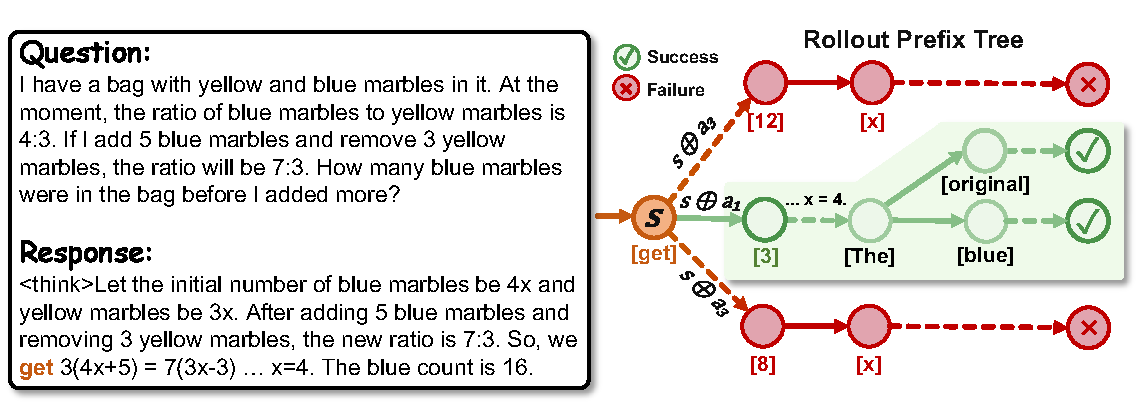
\includegraphics[width=0.98\linewidth]{figure/method.pdf}
\caption{
Illustration of the prefix-tree construction.
Each rollout forms a root-to-leaf path, and shared prefixes are merged into
common nodes.
}
\label{fig:pruned_prefix_tree}
\end{figure}

\paragraph{Positive supervision: reliable prefixes and distributional alignment.}
Following the analysis in Sec.~\ref{sec:ratio_feasibility}, the accuracy and
stability of $\widehat q(a\mid s)$ improve with the number of successful rollouts
passing through $s$.  We therefore retain only prefixes with sufficient successful
support:
\begin{equation}
\mathcal{S}^{+}(x)=\bigl\{s:K(s)\ge m\bigr\},
\label{eq:reliable_prefixes}
\end{equation}
where $m$ is a minimum-success threshold.
On these reliable prefixes, we fit the current policy to the estimated
token-level optimal distribution. The positive loss is
\begin{equation}
\mathcal{L}_{\mathrm{pos}}(\theta)
=
\frac{1}{|\mathcal{B}^{+}|}
\sum_{x}\sum_{s\in\mathcal{S}^{+}(x)}
D_{\mathrm{KL}}\!\bigl(\widehat q(\cdot\mid s)\;\big\|\;\pi_\theta(\cdot\mid s)\bigr),
\label{eq:positive_loss}
\end{equation}
where $|\mathcal{B}^{+}|=\sum_{x}|\mathcal{S}^{+}(x)|$ is the total number of
reliable prefixes in the batch.

\paragraph{Negative supervision: failure frontier and localized penalty.}
In group-based policy optimization methods, trajectories whose rewards fall below the group average receive negative group-relative advantages. These advantages are converted into negative gradient coefficients, producing a negative gradient that is applied uniformly to all tokens in the failed trajectory. We summarize the gradient coefficients of common group-based policy optimization methods in Appendix~\ref{app:objective-gradient-coefficient}.
This trajectory-level penalty is not fully consistent with the error structure of
reasoning tasks, where an incorrect answer is often caused by a small number of
critical decisions rather than every token in the chain \citep{lin2025critical}.
We therefore identify local actions that mark the entrance of a pure-failure subtree.  Specifically, we define the failure frontier
\begin{equation}
\mathcal{F}(x)
=
\bigl\{(s,a):\;K(s)\ge k_{\min},\;
K(s\oplus a)=0,\;
N(s\oplus a)\ge n_{\min}\bigr\},
\label{eq:frontier_set}
\end{equation}
where $k_{\min}$ is a minimum successful-support requirement on the parent prefix
and $n_{\min}$ is a minimum exploration count on the child branch.
The condition $K(s)\ge k_{\min}$ ensures that the parent prefix resides in a
region with demonstrated successful support; $K(s\oplus a)=0$ together with
$N(s\oplus a)\ge n_{\min}$ certifies that the branch entered by action $a$ has
been sufficiently explored yet yields no successful outcome.
On this frontier we apply a unlikelihood penalty that suppresses only
the first statistically certified failure action:
\begin{equation}
\mathcal{L}_{\mathrm{neg}}(\theta)
=
-\frac{1}{|\mathcal{F}|}
\sum_{x}\sum_{(s,a)\in\mathcal{F}(x)}
\log\bigl(1-\pi_\theta(a\mid s)\bigr),
\label{eq:negative_loss}
\end{equation}
where $|\mathcal{F}|=\sum_{x}|\mathcal{F}(x)|$.
By concentrating the penalty on the entrance edge of each pure-failure subtree,
Eq.~\eqref{eq:negative_loss} retains the suppression effect of negative-advantage
updates.
It also avoids over-penalizing downstream tokens, since those tokens are already
conditioned on an earlier erroneous decision.

\paragraph{Combined loss.}
The final training objective combines positive distributional alignment with frontier suppression:
\begin{equation}
\mathcal{L}(\theta)
=
\mathcal{L}_{\mathrm{pos}}(\theta)
+
\gamma\,\mathcal{L}_{\mathrm{neg}}(\theta),
\label{eq:total_loss}
\end{equation}
where $\gamma\ge 0$ balances the two terms.
The resulting signal is critic-free yet dense at the token level: reliable prefixes align the current policy with the estimated token-level optimal distribution obtained from the prefix-tree estimator, while failure-frontier edges contribute localized negative updates that suppress statistically certified failure actions.


\section{Experiments}

\noindent \textbf{Experimental setup.}
We evaluate our method on mathematical reasoning tasks using DeepSeek-R1-Distill-Qwen-1.5B~\citep{deepseekr1} as the backbone. 
Training is conducted on the Big-Math-RL-Verified-Processed dataset~\citep{bigmathverified}. 
We use MATH-500 as the primary benchmark, and additionally evaluate on GSM8K and AIME24 to cover mathematical reasoning tasks with different difficulty levels. 
We compare our method against five representative RL algorithms: GRPO, DAPO, Dr.\ GRPO, GSPO, and SAPO. 
In addition to the binary outcome reward, we use a small auxiliary format reward to encourage standardized final-answer formatting, which improves answer extraction for correctness evaluation. 
We report the average accuracy over three independent seeds on MATH-500, GSM8K, and AIME24
Detailed rewards design, prompt template, hyperparameters, and implementation settings are provided in Appendix~\ref{app:exp_details}.

\noindent \textbf{Curriculum and context schedule.}
As shown in Section~\ref{sec:ratio_feasibility}, reliable estimation of the token-level optimal distribution requires sufficient successful rollouts at each prefix. We therefore adopt an easy-to-hard curriculum based on dataset difficulty partitions to maintain sufficient success coverage throughout training.
To cover both short and long-CoT regimes, we adopt a two-stage answer-length schedule, first training with a 2K maximum response length and then continuing from the resulting checkpoint with a 4K maximum response length. Details are in Appendix~\ref{app:exp_details}.

\noindent \textbf{Result analysis at 2K.}
At the 2K stage, TFPO consistently outperforms all baselines in training dynamics (Figure~\ref{fig:2k_dynamics}) and achieves the best accuracy under the same maximum response length (Table~\ref{tab:short_cot_main}). The advantage emerges early and remains stable throughout training, suggesting that TFPO provides a more efficient optimization signal in the short-CoT regime. This is consistent with our design: TFPO estimates a token-level optimal distribution and directly fits the policy toward this distribution, rather than uniformly assigning a response-level learning signal to all tokens.

\begin{figure}[!htbp]
\centering
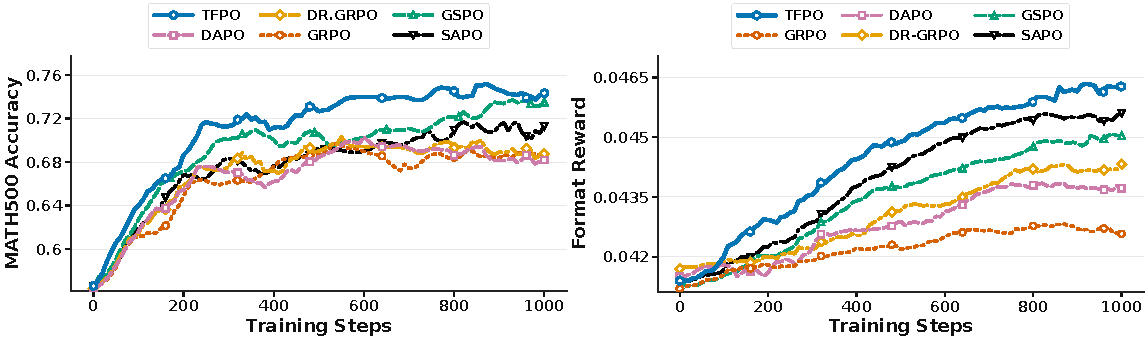
\includegraphics[width=\linewidth]{figure/2k_training_dynamics.pdf}
\vspace{-15pt}
\caption{Training dynamics in the 2K stage. Left: MATH-500 accuracy during training. Right: format reward during training.}
\label{fig:2k_dynamics}
\end{figure}


\begin{table}[htbp]
\centering
\footnotesize
\setlength{\tabcolsep}{2.5pt}
\renewcommand{\arraystretch}{1.0}
\caption{Best accuracy (mean $\pm$ std over 3 seeds) in the short-CoT setting under matched-budget and 32K evaluation.}
\label{tab:short_cot_main}
\begin{tabular*}{\textwidth}{@{\extracolsep{\fill}}l *{6}{c}}
\toprule
\multirow{2}{*}{Method}
& \multicolumn{2}{c}{MATH-500}
& \multicolumn{2}{c}{AIME24}
& \multicolumn{2}{c}{GSM8K} \\
\cmidrule(lr){2-3}
\cmidrule(lr){4-5}
\cmidrule(lr){6-7}
& {2K} & {32K} & {2K} & {32K} & {2K} & {32K} \\
\midrule
Base    & \val{0.564}{0.006} & \val{0.832}{0.004} & \val{0.067}{0.033} & \val{0.267}{0.033} & \val{0.760}{0.001} & \val{0.780}{0.001} \\
\midrule
GRPO    & \val{0.708}{0.006} & \val{0.832}{0.004} & \val{0.033}{0.000} & \val{0.300}{0.000} & \val{0.770}{0.002} & \val{0.782}{0.001} \\
DR-GRPO & \val{0.714}{0.004} & \val{0.834}{0.006} & \val{0.033}{0.000} & \val{0.333}{0.033} & \val{0.768}{0.001} & \val{0.788}{0.001} \\
DAPO    & \val{0.712}{0.004} & \val{0.840}{0.004} & \val{0.067}{0.000} & \val{0.333}{0.000} & \val{0.772}{0.001} & \val{0.788}{0.001} \\
GSPO    & \secondv{0.740}{0.006} & \bestv{0.844}{0.002} & \secondv{0.100}{0.033} & \secondv{0.367}{0.000} & \secondv{0.790}{0.002} & \secondv{0.790}{0.002} \\
SAPO    & \val{0.724}{0.004} & \secondv{0.842}{0.002} & \val{0.067}{0.000} & \val{0.333}{0.000} & \val{0.784}{0.002} & \val{0.788}{0.001} \\
\midrule
\textbf{Ours} & \bestv{0.762}{0.004} & \secondv{0.842}{0.004} & \bestv{0.133}{0.000} & \bestv{0.400}{0.033} & \bestv{0.798}{0.002} & \bestv{0.800}{0.001} \\
\bottomrule
\end{tabular*}
\vspace{-5pt}
\end{table}

To understand the relative ordering among baselines, we examine their gradient
coefficients (Appendix~\ref{app:objective-gradient-coefficient}). 
GRPO assigns a uniform trajectory-level advantage to all tokens, leaving credit assignment coarse under binary outcome reward. 
DAPO and Dr.\ GRPO introduce token-level importance ratios, but their gradient coefficients remain products of clipped token-level ratios and trajectory-level advantages, making optimization sensitive to ratio fluctuation and clipping saturation. 
GSPO and SAPO address this from different angles: GSPO adopts a sequence-level ratio so that all tokens share a coherent coefficient, while SAPO replaces hard clipping with a smooth gate that preserves more gradient signal.
This explains their stronger performance among the baselines. 
Nevertheless, these methods still mainly update tokens indirectly through trajectory-level advantages.
TFPO directly estimates and fits a token-level optimal distribution, providing a more explicit token-level target for policy optimization.




\noindent \textbf{Result analysis at 4K.}
At the 4K stage, TFPO remains the strongest overall method (Table~\ref{tab:long_cot_main}). 
It achieves the best MATH-500 accuracy under both 4K and 32K maximum response lengths, ties for the best AIME24 accuracy at 4K, and obtains the best AIME24 accuracy at 32K. 
The training dynamics in Figure~\ref{fig:4k_dynamics} further support this observation. 
MATH-500 accuracy continues to improve steadily during the 4K stage, showing that the model still benefits from additional optimization under a longer answer-length budget. 
In contrast, the format reward changes only marginally, which is expected because the 4K phase is initialized from the 2K checkpoint, where most answer-formatting behavior has already been learned. 
Thus, the main gain of the 4K stage comes from improving reasoning correctness rather than refining output format.

\begin{figure}[htbp]
\centering
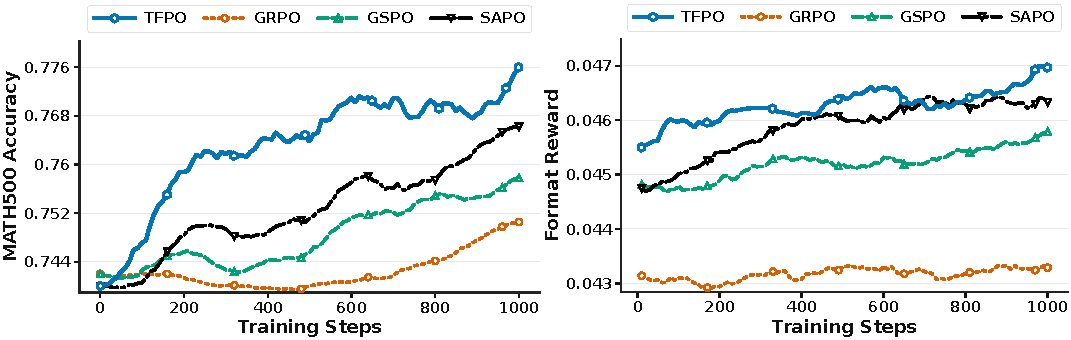
\includegraphics[width=\linewidth]{figure/4k_training_dynamics.pdf}
\vspace{-15pt}
\caption{Training dynamics in the 4K stage. Left: MATH-500 accuracy during training. Right: format reward during training.}
\label{fig:4k_dynamics}
\end{figure}


\begin{table}[htbp]
\centering
\footnotesize
\setlength{\tabcolsep}{2.5pt}
\renewcommand{\arraystretch}{1.0}
\caption{Best accuracy (mean $\pm$ std over 3 seeds) in the long-CoT setting under matched-budget and 32K evaluation.}
\label{tab:long_cot_main}
\begin{tabular*}{\textwidth}{@{\extracolsep{\fill}}l *{6}{c}}
\toprule
\multirow{2}{*}{Method}
& \multicolumn{2}{c}{MATH-500}
& \multicolumn{2}{c}{AIME24}
& \multicolumn{2}{c}{GSM8K} \\
\cmidrule(lr){2-3}
\cmidrule(lr){4-5}
\cmidrule(lr){6-7}
& {4K} & {32K} & {4K} & {32K} & {4K} & {32K} \\
\midrule
Base    & \val{0.738}{0.006} & \val{0.832}{0.002} & \secondv{0.167}{0.033} & \val{0.267}{0.000} & \val{0.764}{0.001} & \val{0.780}{0.001} \\
\midrule
GRPO    & \val{0.754}{0.004} & \val{0.840}{0.004} & \secondv{0.167}{0.000} & \val{0.333}{0.033} & \val{0.764}{0.001} & \val{0.780}{0.001} \\
GSPO    & \val{0.764}{0.006} & \secondv{0.844}{0.002} & \bestv{0.200}{0.033} & \secondv{0.367}{0.000} & \val{0.782}{0.002} & \secondv{0.784}{0.001} \\
SAPO    & \secondv{0.772}{0.004} & \val{0.842}{0.002} & \bestv{0.200}{0.000} & \val{0.333}{0.000} & \secondv{0.784}{0.002} & \secondv{0.784}{0.001} \\
\midrule
\textbf{Ours} & \bestv{0.788}{0.004} & \bestv{0.848}{0.002} & \bestv{0.200}{0.000} & \bestv{0.433}{0.033} & \bestv{0.790}{0.002} & \bestv{0.792}{0.001} \\
\bottomrule
\end{tabular*}
\vspace{-5pt}
\end{table}

A notable exception is GSM8K, where the 4K-stage accuracy is slightly lower
than its 2K counterpart. 
As shown in Figure~\ref{fig:avg_len_2k4k}, the average completion length on GSM8K remains nearly unchanged between 2K and 4K training, suggesting that GSM8K problems make little use of the additional context budget.
Given that the training data contains substantially harder problems while the
model capacity is limited, continuing training at 4K primarily benefits
harder benchmarks such as MATH-500 and AIME24. 
The slight drop on GSM8K is therefore better understood as a capacity trade-off toward high-difficulty reasoning. 


\begin{figure}[htbp]
\centering
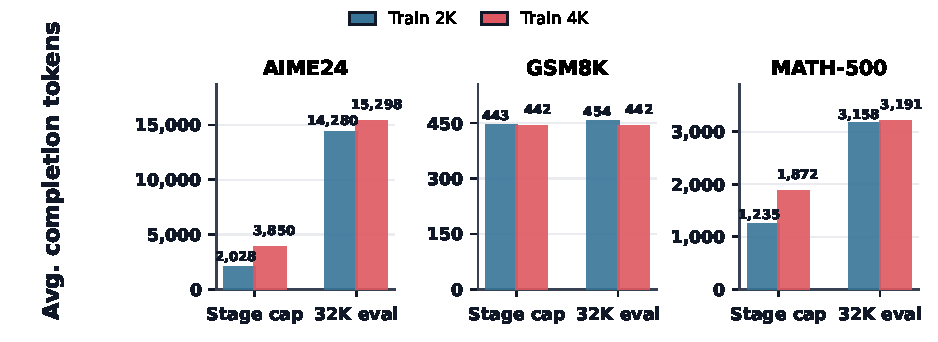
\includegraphics[width=0.95\linewidth]{figure/response_length_2.pdf}
\caption{Average completion length under 2K and 4K training, evaluated under both the stage cap and 32K evaluation budget.}
\label{fig:avg_len_2k4k}
\end{figure}

\noindent \textbf{Ablation study.}
We ablate the two main design choices of TFPO on MATH-500 in the 2K stage: the minimum-success threshold $m$ that determines prefix reliability (Eq.~\ref{eq:reliable_prefixes}), and the negative supervision via the failure-frontier loss $\mathcal{L}_{\mathrm{neg}}$ (Eq.~\ref{eq:negative_loss}). 
We compare full TFPO with three variants: $m=1$, which accepts any prefix with at least one successful rollout; $m=16$, which uses a strict reliability threshold; and w/o neg sup, which removes the penalty by setting $\gamma=0$.

Figure~\ref{fig:ablation} reports the training dynamics and best MATH-500 accuracy.
The threshold $m$ directly controls the reliability of the estimated token-level optimal distribution $\widehat q(a\mid s)$.
With $m=1$, almost any prefix with one successful rollout is used for positive supervision.
This admits many high-variance estimates and leads to weak improvement.
Increasing the threshold to $m=16$ improves filtering, but the estimates remain less reliable than those used by full TFPO.
These results show that TFPO benefits from a sufficiently large success threshold, which provides a more reliable token-level learning signal.

Removing the failure-frontier penalty ($\gamma=0$) reduces best accuracy from 0.766 to 0.732. Without $\mathcal{L}_{\mathrm{neg}}$, the policy still benefits from positive distributional fitting on reliable prefixes but lacks a mechanism to explicitly suppress statistically certified failure actions. The gap shows that localized negative supervision provides a complementary signal that further sharpens the policy's discrimination between correct and erroneous token-level decisions.

\begin{figure}[t]
\centering
\vspace{-5pt}
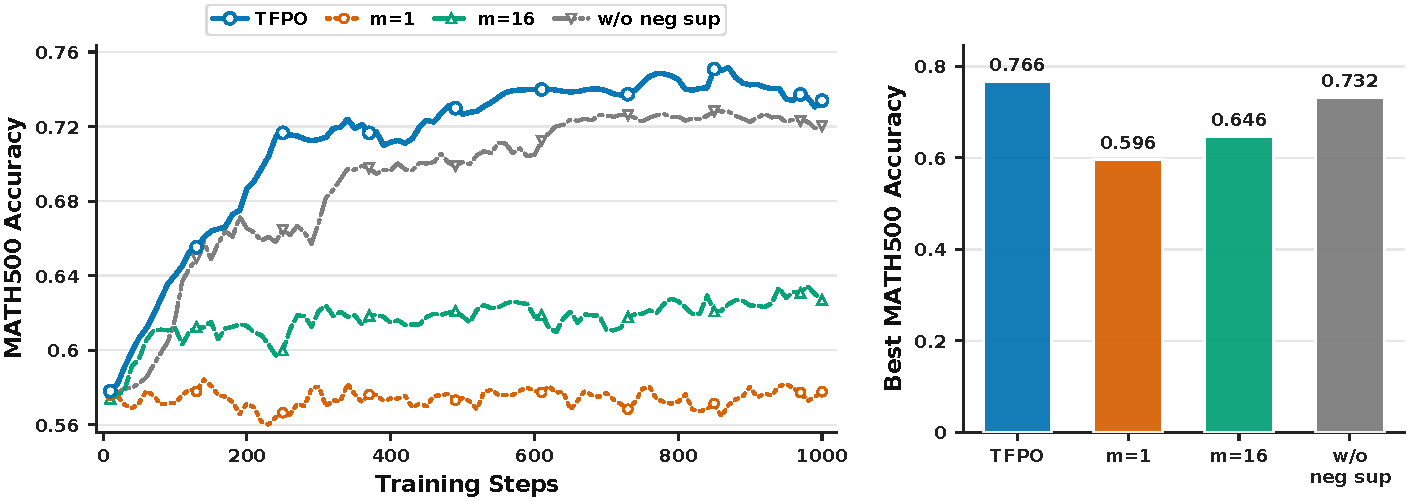
\includegraphics[width=0.95\linewidth]{figure/combined_step_acc_plot.pdf}
\vspace{-8pt}
\caption{Ablation study on MATH-500 in the 2K stage. Left: training dynamics of each variant. Right: best accuracy achieved over training. }
\label{fig:ablation}
\end{figure}


\section{Conclusion}
We proposed TFPO, a policy optimization method that derives a token-level optimal distribution from the KL-regularized RL objective and fits the current policy to it using only binary outcome reward.
By conditioning the trajectory-level optimal distribution on prefixes, the intractable global partition function cancels exactly, and reliable estimation requires only a moderate number of successful rollouts per prefix. 
TFPO is fully compatible with GRPO-style algorithms and consistently outperforms representative baselines on GSM8K, MATH-500, and AIME24, with especially notable gains on the more challenging benchmarks.

\bibliographystyle{unsrtnat}
\bibliography{references}



\appendix
\section{Related Work}

\subsection{Reasoning RL Algorithms}

PPO~\citep{ppo} is the standard optimizer for RLHF~\citep{NEURIPS2022_b1efde53}, but its reliance on a critic of comparable scale to the policy makes training memory-intensive and prone to instability. GRPO~\citep{shao2024deepseekmath} removes the critic by computing advantages from group-relative rewards over multiple rollouts of the same prompt, and has become the standard backbone for reasoning RL. Several refinements have been proposed: Dr.~GRPO~\citep{liu2025drgrpo} corrects the length bias in GRPO's normalization; DAPO~\citep{yu2025dapo} decouples the upper and lower clipping thresholds and dynamically resamples prompts whose rollouts yield identical rewards; GSPO~\citep{zhang2025gspo} reformulates importance weighting at the sequence level; and SAPO~\citep{wang2025sapo} replaces the hard PPO clip with a smooth adaptive gate. Although DAPO and Dr.~GRPO modulate updates with token-level importance ratios, the advantage that drives the gradient is still computed once per trajectory and shared across every token, leaving credit assignment coarse under binary outcome reward.

\subsection{Credit Assignment}

In long-CoT reasoning, an incorrect final answer is often caused by only a few critical tokens rather than the chain as a whole~\citep{lin2025critical}, which makes coarse credit assignment particularly problematic.
A widely studied solution is to introduce step- or token-level supervision through auxiliary models. \citet{lightman2023letsverify} demonstrate that step-level Process Reward Models (PRMs) substantially outperform outcome-only supervision in mathematical reasoning. Math-Shepherd~\citep{wang2024mathshepherdverifyreinforcellms} and OmegaPRM~\citep{luo2024automated} avoid manual step annotation by deriving process labels from Monte Carlo rollouts, while Token-Supervised Value Models~\citep{lee2025tvm} push granularity to the token level and Step-DPO~\citep{xu-etal-2025-full} aligns preference optimization with the first erroneous reasoning step. Such methods deliver dense supervision but require training a separate verifier or value model, which adds system complexity and an additional source of estimation error. Self-training methods including STaR~\citep{NEURIPS2022_639a9a17}, ReST~\citep{Gulcehre2023ReinforcedS}, and ReST$^{\text{EM}}$~\citep{Singh2023BeyondHD} sidestep this overhead by fine-tuning on filtered correct trajectories, but discard failed rollouts entirely and provide no localized signal for where errors originate.

A more recent line aims to recover token- or step-level signals from outcome reward without any auxiliary model. VinePPO~\citep{kazemnejad2025vinepporefiningcreditassignment} estimates per-token values via Monte Carlo continuations from each prefix and uses them in a standard PPO update. Implicit PRM~\citep{yuan2024freeprocessrewardsprocess} and PRIME~\citep{cui2025processreinforcementimplicitrewards} derive process rewards from a specific parameterization of the outcome reward, providing dense online feedback during training. Critical Token Optimization~\citep{lin2025critical} identifies decisive tokens via contrastive estimation and concentrates updates on them. Tree-search methods such as ReST-MCTS*~\citep{zhang2024rest} and rStar-Math~\citep{guan2025rstarmathsmallllmsmaster} integrate MCTS into the rollout procedure to assign step-level values. Our work belongs to this category but estimates a token-level conditional distribution derived from the KL-regularized RL objective, rather than a scalar value or advantage that is then consumed by a policy-gradient surrogate.

\section{Limitations}
First, TFPO relies on sufficient successful rollouts at each prefix to construct reliable token-level optimal distribution estimates. When the success rate is low, the set of reliable prefixes may become sparse. To address this, we adopt an easy-to-hard curriculum to maintain adequate success coverage, and failed rollouts are further exploited through the failure-frontier penalty in Eq.~\eqref{eq:negative_loss}. Since TFPO and group-based policy optimization methods share the same KL-regularized policy optimization objective, investigating whether the two can be combined to further exploit unreliable prefixes is a promising direction for future work. 

Second, our experiments are limited to DeepSeek-R1-Distill-Qwen-1.5B on mathematical reasoning. Since our theory is independent of model scale and task domain, TFPO may further benefit from larger models, as their higher success rates could provide denser reliable prefixes and broader token-level coverage. Testing this expectation on larger models and extending TFPO to other reasoning domains, such as code generation, are important directions for future work.

Finally, TFPO extracts token-level signals purely from binary outcome reward, while process reward models leverage step-level annotations. These two approaches address credit assignment from complementary angles, and investigating whether their combination yields further improvements is a promising future direction.

\section{Sample Complexity of Direct Monte Carlo Estimation of the Partition Function}
\label{app:z_estimation}

In this appendix, we quantify why the trajectory-level optimal distribution in Eq.~\eqref{eq:traj_opt} is difficult to use directly under sparse terminal rewards. The issue is that evaluating $\pi^\star(y \mid x)$ requires estimating the partition function
\begin{equation}
Z_\rho(x)
:=
\mathbb{E}_{y \sim \rho(\cdot \mid x)}
\left[
\exp\!\left(\frac{R(x,y)}{\beta}\right)
\right].
\label{eq:appendix_partition_def}
\end{equation}
We show that, under sparse terminal rewards, the variance of its direct Monte Carlo estimator grows exponentially as $\beta \to 0$.

\paragraph{Setup.}
Fix a prompt $x$ and assume the terminal reward is binary:
\begin{equation}
R(x,y) \in \{0,1\}.
\end{equation}
Define
\begin{equation}
p_x := \Pr_{y \sim \rho(\cdot \mid x)}[R(x,y)=1],
\qquad
c := \exp(1/\beta).
\end{equation}
Then the exponential weight
\begin{equation}
w(x,y) := \exp\!\left(\frac{R(x,y)}{\beta}\right)
\end{equation}
takes values in $\{1,c\}$, and Eq.~\eqref{eq:appendix_partition_def} becomes
\begin{equation}
Z_\rho(x)
=
\mathbb{E}_{y \sim \rho(\cdot \mid x)}[w(x,y)]
=
1 + p_x(c-1).
\label{eq:appendix_partition_binary}
\end{equation}

Given $G$ i.i.d.\ samples $y^{(1)},\ldots,y^{(G)} \sim \rho(\cdot \mid x)$, consider the direct Monte Carlo estimator
\begin{equation}
\widehat{Z}_\rho(x)
:=
\frac{1}{G}\sum_{i=1}^G
\exp\!\left(\frac{R(x,y^{(i)})}{\beta}\right)
=
\frac{1}{G}\sum_{i=1}^G w(x,y^{(i)}).
\label{eq:appendix_z_hat}
\end{equation}

\begin{proposition}
\label{prop:z_variance}
The estimator $\widehat{Z}_\rho(x)$ is unbiased and satisfies
\begin{equation}
\mathrm{Var}\!\left[\widehat{Z}_\rho(x)\right]
=
\frac{(c-1)^2}{G}\,p_x(1-p_x).
\label{eq:appendix_z_variance}
\end{equation}
In particular, if $p_x(1-p_x)=\Theta(1)$, then
\begin{equation}
\mathrm{Var}\!\left[\widehat{Z}_\rho(x)\right]
=
\Theta\!\left(\frac{(e^{1/\beta}-1)^2}{G}\right)
=
\Theta\!\left(\frac{e^{2/\beta}}{G}\right).
\label{eq:appendix_z_variance_asym}
\end{equation}
\end{proposition}

\begin{proof}
Unbiasedness follows from linearity of expectation:
\begin{equation}
\mathbb{E}[\widehat{Z}_\rho(x)]
=
\frac{1}{G}\sum_{i=1}^G \mathbb{E}[w(x,y^{(i)})]
=
\mathbb{E}_{y \sim \rho(\cdot \mid x)}[w(x,y)]
=
Z_\rho(x).
\end{equation}

Since the samples are i.i.d.,
\begin{equation}
\mathrm{Var}\!\left[\widehat{Z}_\rho(x)\right]
=
\frac{1}{G}\mathrm{Var}[w(x,y)].
\label{eq:appendix_var_mean}
\end{equation}
Moreover, $w(x,y)=c$ with probability $p_x$ and $w(x,y)=1$ with probability $1-p_x$, so
\begin{equation}
\mathbb{E}[w(x,y)^2]
=
(1-p_x)\cdot 1^2 + p_x \cdot c^2
=
1 + p_x(c^2-1).
\end{equation}
Combining this with Eq.~\eqref{eq:appendix_partition_binary}, we obtain
\begin{align}
\mathrm{Var}[w(x,y)]
&=
\mathbb{E}[w(x,y)^2] - \mathbb{E}[w(x,y)]^2 \\
&=
\left(1 + p_x(c^2-1)\right) - \left(1 + p_x(c-1)\right)^2 \\
&=
p_x(1-p_x)(c-1)^2.
\end{align}
Substituting into Eq.~\eqref{eq:appendix_var_mean} yields Eq.~\eqref{eq:appendix_z_variance}. The asymptotic form in Eq.~\eqref{eq:appendix_z_variance_asym} follows from $c=e^{1/\beta}$.
\end{proof}

\begin{corollary}
\label{cor:z_sample_complexity}
For any $\varepsilon > 0$ and $\delta \in (0,1)$,
\begin{equation}
\Pr\!\left(
\left|\widehat{Z}_\rho(x)-Z_\rho(x)\right| \ge \varepsilon
\right)
\le
\frac{(c-1)^2 p_x(1-p_x)}{G \varepsilon^2}.
\label{eq:appendix_chebyshev}
\end{equation}
Hence, it suffices to choose
\begin{equation}
G
\ge
\frac{(c-1)^2 p_x(1-p_x)}{\delta \varepsilon^2}
\label{eq:appendix_sample_complexity}
\end{equation}
to ensure
\begin{equation}
\Pr\!\left(
\left|\widehat{Z}_\rho(x)-Z_\rho(x)\right| \ge \varepsilon
\right)
\le \delta.
\end{equation}
In particular, if $p_x(1-p_x)=\Theta(1)$, then it suffices to take
\begin{equation}
G
=
\Theta\!\left(\frac{(e^{1/\beta}-1)^2}{\delta \varepsilon^2}\right)
=
\Theta\!\left(\frac{e^{2/\beta}}{\delta \varepsilon^2}\right).
\label{eq:appendix_sample_complexity_asym}
\end{equation}
\end{corollary}

\begin{proof}
By Chebyshev's inequality and Proposition~\ref{prop:z_variance},
\begin{equation}
\Pr\!\left(
\left|\widehat{Z}_\rho(x)-Z_\rho(x)\right| \ge \varepsilon
\right)
\le
\frac{\mathrm{Var}[\widehat{Z}_\rho(x)]}{\varepsilon^2}
=
\frac{(c-1)^2 p_x(1-p_x)}{G \varepsilon^2},
\end{equation}
which proves Eq.~\eqref{eq:appendix_chebyshev}. To guarantee
\begin{equation}
\Pr\!\left(
\left|\widehat{Z}_\rho(x)-Z_\rho(x)\right| \ge \varepsilon
\right)
\le \delta,
\end{equation}
it is therefore sufficient to require that
\begin{equation}
\frac{(c-1)^2 p_x(1-p_x)}{G \varepsilon^2} \le \delta.
\end{equation}
Rearranging gives
\begin{equation}
G \ge \frac{(c-1)^2 p_x(1-p_x)}{\delta \varepsilon^2},
\end{equation}
establishing Eq.~\eqref{eq:appendix_sample_complexity}. Finally, when $p_x(1-p_x)=\Theta(1)$ and $c=e^{1/\beta}$,
\begin{equation}
\frac{(c-1)^2 p_x(1-p_x)}{\delta \varepsilon^2}
=
\Theta\!\left(\frac{(e^{1/\beta}-1)^2}{\delta \varepsilon^2}\right)
=
\Theta\!\left(\frac{e^{2/\beta}}{\delta \varepsilon^2}\right),
\end{equation}
which establishes Eq.~\eqref{eq:appendix_sample_complexity_asym}.
\end{proof}

\paragraph{Interpretation.}
From Corollary~\ref{cor:z_sample_complexity}, the sample complexity of direct Monte Carlo estimation of $Z_\rho(x)$ under binary outcome reward scales as $\Theta\!\left(e^{2/\beta}/(\delta \varepsilon^2)\right)$. Therefore, obtaining an accurate estimate of the global partition function requires a number of rollouts that grows exponentially in $1/\beta$. For the relatively small values of $\beta$ commonly used in practice, this sample requirement is prohibitively large. Consequently, under realistic rollout budgets, $Z_\rho(x)$ cannot be estimated accurately enough for stable trajectory-level fitting, making the trajectory-level optimal distribution in Eq.~\eqref{eq:traj_opt} impractical to use directly.


\section{Derivation of the Token-Level Optimal Distribution}
\label{app:token_opt_derivation}

We prove Theorem~\ref{thm:token_level_optimal_distribution}. Starting from the definition of the prefix-conditioned next-token distribution,
\begin{equation}
q^\star(a \mid s)
=
\frac{\sum_{y:\, s \oplus a \preceq y}\pi^\star(y \mid x)}
{\sum_{y:\, s \preceq y}\pi^\star(y \mid x)}.
\end{equation}
Substituting the trajectory-level optimum in Eq.~\eqref{eq:traj_opt} gives
\begin{align}
q^\star(a \mid s)
&=
\frac{
\sum_{y:\, s \oplus a \preceq y}
\frac{1}{Z_\rho(x)}\rho(y \mid x)
\exp\!\left(\frac{R(x,y)}{\beta}\right)
}{
\sum_{y:\, s \preceq y}
\frac{1}{Z_\rho(x)}\rho(y \mid x)
\exp\!\left(\frac{R(x,y)}{\beta}\right)
}
\nonumber\\
&=
\frac{
\sum_{y:\, s \oplus a \preceq y}
\rho(y \mid x)
\exp\!\left(\frac{R(x,y)}{\beta}\right)
}{
\sum_{y:\, s \preceq y}
\rho(y \mid x)
\exp\!\left(\frac{R(x,y)}{\beta}\right)
}.
\end{align}
Thus, the global partition function $Z_\rho(x)$ cancels exactly. Finally, for any prefix $u$,
\begin{equation}
\sum_{y:\, u \preceq y}
\rho(y \mid x)
\exp\!\left(\frac{R(x,y)}{\beta}\right)
=
\mathbb{E}_{y \sim \rho(\cdot \mid x)}
\!\left[
\exp\!\left(\frac{R(x,y)}{\beta}\right)
\mathbb{I}[u \preceq y]
\right].
\end{equation}
Applying this identity to $u=s\oplus a$ and $u=s$ proves Eq.~\eqref{eq:token_opt_ratio_expectation}.



\section{Consistency and Local Sample Complexity of the Ratio Estimator}
\label{app:ratio_consistency}

We reuse the notation from Sec.~\ref{sec:token_opt_distribution}. For compactness,
write the population prefix mass in Eq.~\eqref{eq:token_opt_ratio_expectation} as
\begin{equation}
M(u)
:=
\mathbb{E}_{y\sim\rho(\cdot\mid x)}
\!\left[
\exp\!\left(\frac{R(x,y)}{\beta}\right)
\mathbb{I}[u\preceq y]
\right],
\end{equation}
and let $\widehat M_G(u)$ be its empirical average over the same rollout batch
used in Eq.~\eqref{eq:token_opt_mc}. Then
\begin{equation}
q^\star(a\mid s)=\frac{M(s\oplus a)}{M(s)},
\qquad
\widehat q(a\mid s)
=
\frac{\widehat M_G(s\oplus a)}{\widehat M_G(s)}.
\end{equation}

\begin{proposition}[Consistency]
\label{prop:ratio_consistency}
Assume $M(s)>0$ and the exponential weight has finite expectation under
$\rho(\cdot\mid x)$. Then
\begin{equation}
\widehat q(a\mid s)
\xrightarrow[]{p}
q^\star(a\mid s)
\qquad \text{as } G\to\infty .
\end{equation}
\end{proposition}

\begin{proof}
By the law of large numbers,
$\widehat M_G(s\oplus a)\xrightarrow[]{p}M(s\oplus a)$ and
$\widehat M_G(s)\xrightarrow[]{p}M(s)$. Since $M(s)>0$, the ratio map is
continuous at $(M(s\oplus a),M(s))$. The continuous mapping theorem gives the
claim.
\end{proof}

The consistency result is asymptotic. We next give the finite-sample statement
used in Sec.~\ref{sec:ratio_feasibility}. Assume binary rewards and set
$c=e^{1/\beta}$. Let $K_u$ and $F_u$ denote the numbers of successful and failed
rollouts that pass through prefix $u$. Define
\begin{equation}
p_s^+
:=
\Pr_{y\sim\rho(\cdot\mid x)}[s\preceq y,\ R(x,y)=1],
\qquad
p_s^-
:=
\Pr_{y\sim\rho(\cdot\mid x)}[s\preceq y,\ R(x,y)=0],
\end{equation}
and the success-conditioned continuation probability
\begin{equation}
q^+(a\mid s)
:=
\Pr_{y\sim\rho(\cdot\mid x)}
[s\oplus a\preceq y \mid s\preceq y,\ R(x,y)=1].
\end{equation}

\begin{proposition}[Local concentration from successful support]
\label{prop:local_success_concentration}
Let $\mathcal{C}(s)$ be a local action set with $d_s=|\mathcal{C}(s)|$.
If $K_s>0$ and $p_s^+>0$, then conditioned on $K_s$ and $F_s$, with probability
at least $1-\delta$,
\begin{equation}
\max_{a\in\mathcal{C}(s)}
\left|
\widehat q(a\mid s)-q^\star(a\mid s)
\right|
\le
\sqrt{\frac{\log(2d_s/\delta)}{2K_s}}
+
\frac{F_s}{cK_s}
+
\frac{p_s^-}{cp_s^+}.
\label{eq:appendix_local_concentration}
\end{equation}
\end{proposition}

\begin{proof}
First consider only successful rollouts through $s$ and define
\begin{equation}
\bar q(a\mid s)
:=
\frac{K_{s\oplus a}}{K_s}.
\end{equation}
Conditioned on $K_s=m$, the indicators for whether each successful rollout
continues with action $a$ are Bernoulli random variables with mean
$q^+(a\mid s)$. Hence Hoeffding's inequality gives
\begin{equation}
\Pr\!\left(
|\bar q(a\mid s)-q^+(a\mid s)|>\eta
\mid K_s=m
\right)
\le
2\exp(-2m\eta^2).
\end{equation}
Taking a union bound over $a\in\mathcal{C}(s)$ and setting
\[
\eta=
\sqrt{\frac{\log(2d_s/\delta)}{2K_s}}
\]
gives, with probability at least $1-\delta$,
\begin{equation}
\max_{a\in\mathcal{C}(s)}
|\bar q(a\mid s)-q^+(a\mid s)|
\le
\sqrt{\frac{\log(2d_s/\delta)}{2K_s}}.
\label{eq:appendix_success_only_concentration}
\end{equation}

It remains to account for failed rollouts. Under binary rewards,
\begin{equation}
\widehat q(a\mid s)
=
\frac{cK_{s\oplus a}+F_{s\oplus a}}{cK_s+F_s}.
\end{equation}
If $F_s=0$, then $\widehat q(a\mid s)=\bar q(a\mid s)$. Otherwise, let
$\bar q^-(a\mid s):=F_{s\oplus a}/F_s$. Then
\begin{equation}
\widehat q(a\mid s)
=
\frac{cK_s}{cK_s+F_s}\bar q(a\mid s)
+
\frac{F_s}{cK_s+F_s}\bar q^-(a\mid s),
\end{equation}
so
\begin{equation}
|\widehat q(a\mid s)-\bar q(a\mid s)|
\le
\frac{F_s}{cK_s+F_s}
\le
\frac{F_s}{cK_s}.
\label{eq:appendix_empirical_failed_term}
\end{equation}

The population target admits the analogous decomposition. Let
\[
q^-(a\mid s)
:=
\Pr[s\oplus a\preceq y \mid s\preceq y,\ R(x,y)=0],
\]
with an arbitrary value if $p_s^-=0$. Then
\begin{equation}
q^\star(a\mid s)
=
\frac{cp_s^+}{cp_s^+ + p_s^-}q^+(a\mid s)
+
\frac{p_s^-}{cp_s^+ + p_s^-}q^-(a\mid s),
\end{equation}
which implies
\begin{equation}
|q^\star(a\mid s)-q^+(a\mid s)|
\le
\frac{p_s^-}{cp_s^+ + p_s^-}
\le
\frac{p_s^-}{cp_s^+}.
\label{eq:appendix_population_failed_term}
\end{equation}
Combining Eqs.~\eqref{eq:appendix_success_only_concentration},
\eqref{eq:appendix_empirical_failed_term}, and
\eqref{eq:appendix_population_failed_term} by the triangle inequality proves
Eq.~\eqref{eq:appendix_local_concentration}.
\end{proof}

\paragraph{Interpretation.}
Proposition~\ref{prop:local_success_concentration} separates the stochastic
success-supported term from the failed-rollout corrections.
The first term decreases as $O(1/\sqrt{K_s})$ with the number of successful
rollouts. The second and third terms are both suppressed by the factor
$c=e^{1/\beta}$: for typical values of $\beta$ used in practice
(e.g.\ $\beta=0.1$, $c\approx 2.2\times 10^4$), they are negligible
compared to the stochastic term.
Therefore, the estimation error is effectively governed by the successful
support $K_s$ and carries no exponential dependence on $1/\beta$.


\section{Variance Analysis of the Ratio Estimator}
\label{app:ratio_estimation}

In this appendix, we derive the variance bound used in Sec.~\ref{sec:ratio_feasibility}. Our goal is to show that, once a prefix $s$ is supported by successful rollouts, the variance of the ratio estimator $\widehat q(a \mid s)$ is controlled primarily by the number of successful sampled trajectories reaching $s$, rather than by the exponential scale $e^{1/\beta}$.

\paragraph{Setup.}
Fix a prompt $x$ and a complete response $y$. Assume binary terminal rewards:
\begin{equation}
R(x,y)\in\{0,1\}.
\end{equation}
Let
\begin{equation}
c := e^{1/\beta}.
\end{equation}
Given $G$ i.i.d.\ samples
\begin{equation}
y^{(1)},\ldots,y^{(G)} \sim \rho(\cdot \mid x),
\end{equation}
define, for any prefix $u$,
\begin{equation}
K_u
:=
\sum_{i=1}^G
\mathbb{I}[u \preceq y^{(i)},\, R(x,y^{(i)})=1],
\qquad
F_u
:=
\sum_{i=1}^G
\mathbb{I}[u \preceq y^{(i)},\, R(x,y^{(i)})=0].
\label{eq:appendix_prefix_counts}
\end{equation}
That is, $K_u$ and $F_u$ are the numbers of successful and failed sampled trajectories passing through prefix $u$, respectively. Under binary rewards, each sampled trajectory contributes either unit weight or exponential weight. Therefore, the ratio estimator can be written as
\begin{equation}
\widehat q(a \mid s)
=
\frac{F_{s\oplus a}+cK_{s\oplus a}}{F_s+cK_s}.
\label{eq:appendix_qhat_counts}
\end{equation}

To derive the variance of $\widehat q(a \mid s)$, it is convenient to compare it with the simpler success-only ratio
\begin{equation}
\bar q(a \mid s)
:=
\frac{K_{s\oplus a}}{K_s},
\qquad \text{whenever } K_s>0.
\label{eq:appendix_qbar}
\end{equation}
This quantity is introduced only as an auxiliary object for the derivation. The idea is to first derive a variance bound for $\bar q(a \mid s)$, and then quantify how much $\widehat q(a \mid s)$ deviates from it due to failed trajectories.

\paragraph{Step 1: Variance of the success-only ratio.}
Condition on $K_s=m\ge 1$. Among the $m$ successful sampled trajectories that pass through prefix $s$, each either continues with token $a$ or not. Since the rollouts are i.i.d., these $m$ indicators are conditionally i.i.d.\ Bernoulli random variables with some parameter $p_{s,a}\in[0,1]$. Therefore,
\begin{equation}
K_{s\oplus a}\mid K_s=m \sim \mathrm{Bin}(m,p_{s,a}).
\label{eq:appendix_binomial}
\end{equation}
Using Eq.~\eqref{eq:appendix_qbar}, we obtain
\begin{equation}
\mathrm{Var}\!\left[\bar q(a \mid s)\mid K_s=m\right]
=
\frac{1}{m^2}\mathrm{Var}\!\left[K_{s\oplus a}\mid K_s=m\right]
=
\frac{p_{s,a}(1-p_{s,a})}{m}
\le
\frac{1}{4m}.
\end{equation}
Hence, whenever $K_s>0$,
\begin{equation}
\mathrm{Var}\!\left[\bar q(a \mid s)\mid K_s\right]
\le
\frac{1}{4K_s}.
\label{eq:appendix_qbar_variance}
\end{equation}

\paragraph{Step 2: Deviation of $\widehat q(a \mid s)$ from $\bar q(a \mid s)$.}
Using Eq.~\eqref{eq:appendix_qhat_counts} and Eq.~\eqref{eq:appendix_qbar},
\begin{align}
\widehat q(a \mid s)-\bar q(a \mid s)
&=
\frac{F_{s\oplus a}+cK_{s\oplus a}}{F_s+cK_s}
-
\frac{K_{s\oplus a}}{K_s}
\nonumber\\
&=
\frac{K_sF_{s\oplus a}-F_sK_{s\oplus a}}
{K_s(F_s+cK_s)}.
\label{eq:appendix_gap_exact}
\end{align}
Since $0\le F_{s\oplus a}\le F_s$ and $0\le K_{s\oplus a}\le K_s$,
\begin{equation}
\left|K_sF_{s\oplus a}-F_sK_{s\oplus a}\right|
\le
K_sF_{s\oplus a}+F_sK_{s\oplus a}
\le
2F_sK_s.
\end{equation}
Substituting this into Eq.~\eqref{eq:appendix_gap_exact} yields
\begin{equation}
\left|
\widehat q(a \mid s)-\bar q(a \mid s)
\right|
\le
\frac{2F_sK_s}{K_s(F_s+cK_s)}
=
\frac{2F_s}{F_s+cK_s}
\le
\frac{2F_s}{cK_s}.
\label{eq:appendix_qhat_qbar_gap}
\end{equation}
Therefore,
\begin{equation}
\mathbb{E}\!\left[
\bigl(\widehat q(a \mid s)-\bar q(a \mid s)\bigr)^2
\mid K_s,F_s
\right]
\le
\frac{4F_s^2}{c^2K_s^2}.
\label{eq:appendix_delta_second_moment}
\end{equation}

\paragraph{Step 3: Variance of the ratio estimator.}

Let
\begin{equation}
\Delta(a \mid s)
:=
\widehat q(a \mid s)-\bar q(a \mid s).
\end{equation}
Then
\begin{equation}
\widehat q(a \mid s)=\bar q(a \mid s)+\Delta(a \mid s).
\end{equation}
Using $\mathrm{Var}(U+V)\le 2\,\mathrm{Var}(U)+2\,\mathrm{Var}(V)$ and $\mathrm{Var}(V)\le \mathbb{E}[V^2]$, we obtain
\begin{align}
\mathrm{Var}\!\left[\widehat q(a \mid s)\mid K_s,F_s\right]
&=
\mathrm{Var}\!\left[\bar q(a \mid s)+\Delta(a \mid s)\mid K_s,F_s\right]
\nonumber\\
&\le
2\,\mathrm{Var}\!\left[\bar q(a \mid s)\mid K_s,F_s\right]
+
2\,\mathrm{Var}\!\left[\Delta(a \mid s)\mid K_s,F_s\right]
\nonumber\\
&\le
2\,\mathrm{Var}\!\left[\bar q(a \mid s)\mid K_s\right]
+
2\,\mathbb{E}\!\left[\Delta(a \mid s)^2 \mid K_s,F_s\right].
\label{eq:appendix_var_decomp}
\end{align}
Applying Eq.~\eqref{eq:appendix_qbar_variance} and Eq.~\eqref{eq:appendix_delta_second_moment} to Eq.~\eqref{eq:appendix_var_decomp} gives
\begin{equation}
\mathrm{Var}\!\left[\widehat q(a \mid s)\mid K_s,F_s\right]
\le
\frac{1}{2K_s}
+
\frac{8F_s^2}{c^2K_s^2}.
\label{eq:appendix_qhat_variance}
\end{equation}

\paragraph{Final variance bound.}
Substituting $c=e^{1/\beta}$ into Eq.~\eqref{eq:appendix_qhat_variance}, we obtain
\begin{equation}
\mathrm{Var}\!\left[\widehat q(a \mid s)\mid K_s,F_s\right]
\le
\frac{1}{2K_s}
+
\frac{8F_s^2}{e^{2/\beta}K_s^2}.
\label{eq:appendix_qhat_variance_beta}
\end{equation}
In particular, once $K_s>0$, the estimator does not exhibit exponential variance blow-up as $\beta\to 0$.

\paragraph{Interpretation.}
Eq.~\eqref{eq:appendix_qhat_variance_beta} shows that the variance of the ratio estimator is governed primarily by the inverse successful-sample count $1/K_s$. The second term is additionally suppressed by $e^{-2/\beta}$. Therefore, unlike direct estimation of $Z_\rho(x)$, the token-level ratio estimator does not suffer exponential variance explosion in the low-temperature regime. This is the formal reason why the token-level estimator remains statistically feasible under sparse terminal rewards, provided that the prefix is supported by successful rollouts.


\section{Hyperparameters and Compute Resources}
\label{app:exp_details}

\paragraph{Compute setup.}
All experiments for our method and the comparison methods were run on two NVIDIA H100 GPUs. One GPU is reserved for policy training, while the other is reserved for inference and evaluation. 

\paragraph{Prompt template.}
For all experiments using the DeepSeek-R1-Distill-Qwen-1.5B backbone, including both our method and the comparison baselines, we use the same DeepSeek-style chat prompt for rollout generation during training and for evaluation:

\begin{center}
\fbox{%
\begin{minipage}{0.94\linewidth}
\small\ttfamily
<|begin of sentence|><|User|> Solve the following math problem efficiently and clearly.
Think step by step before answering. Put the final answer at the very end of your
response using exactly this format: Therefore, the final answer is:
\$\textbackslash boxed\{\{your answer\}\}\$. I hope it is correct.

\{problem\}

<|Assistant|><think>
\end{minipage}%
}
\end{center}

This prompt is designed to elicit step-by-step reasoning and to enforce that the final answer appears in boxed form, which is consistent with our answer extraction pipeline and the format reward used in training.


\paragraph{Reward design and answer extraction.}
Training uses an outcome-based reward together with a small auxiliary format reward. The outcome reward is binary: a response receives 1 if the extracted final answer matches the reference answer, and 0 otherwise. To improve extraction reliability, we instruct the model to place its final answer inside \texttt{\textbackslash boxed\{\}} and assign a format reward of 0.05 when the final answer is presented in the required boxed form; otherwise, the format reward is 0.



\paragraph{Curriculum and context schedule details.}
The easy-to-hard curriculum is implemented using the five dataset-defined difficulty partitions of Big-Math-RL-Verified-Processed, denoted by \texttt{level\_1} to \texttt{level\_5}, where the levels are constructed from quintiles of \texttt{llama8b\_solve\_rate}. Here, \texttt{level\_1} corresponds to the easiest subset and \texttt{level\_5} to the hardest. In both training phases, we use a stage-wise sampling schedule over these five levels, as summarized in Table~\ref{tab:curriculum_schedule}. Phase 1 corresponds to the 2K stage, and Phase 2 corresponds to the 4K stage. This schedule gradually shifts training from easier to harder problems, while maintaining sufficient success coverage for constructing reliable local supervision throughout optimization.

\begin{table}[htbp]
\centering
\small
\setlength{\tabcolsep}{4.5pt}
\renewcommand{\arraystretch}{1.1}
\begin{tabular}{llccccc}
\toprule
Phase & Iterations & \texttt{level\_1} & \texttt{level\_2} & \texttt{level\_3} & \texttt{level\_4} & \texttt{level\_5} \\
\midrule
\multirow{3}{*}{Phase 1 (2K)}
& 1--300    & 0.40 & 0.35 & 0.15 & 0.05 & 0.05 \\
& 301--600  & 0.20 & 0.20 & 0.35 & 0.15 & 0.10 \\
& 601--1000 & 0.05 & 0.05 & 0.20 & 0.30 & 0.40 \\
\midrule
\multirow{3}{*}{Phase 2 (4K)}
& 1--300    & 0.25 & 0.20 & 0.30 & 0.15 & 0.10 \\
& 301--600  & 0.10 & 0.10 & 0.30 & 0.20 & 0.30 \\
& 601--1000 & 0.03 & 0.02 & 0.15 & 0.30 & 0.50 \\
\bottomrule
\end{tabular}
\caption{Stage-wise sampling weights for the easy-to-hard curriculum in the 2K and 4K training phases.}
\label{tab:curriculum_schedule}
\end{table}

\FloatBarrier

\paragraph{Hyperparameter summary.}
Table~\ref{tab:main_hparams_all} summarizes the key hyperparameters of our method and the baselines in the 2K and 4K training phases.

\begin{table}[htbp]
\centering
\scriptsize
\setlength{\tabcolsep}{3.5pt}
\renewcommand{\arraystretch}{1.08}
\begin{tabular*}{\textwidth}{@{\extracolsep{\fill}}lcccccc}
\toprule
Hyperparameter & Ours & GRPO & DR-GRPO & DAPO & GSPO & SAPO \\
\midrule

\multicolumn{7}{c}{\textbf{2K phase}} \\
\midrule
$\beta$ & 0.1 & 0.1 & 0.1 & 0.1 & 0.1 & 0.1 \\
Success threshold $m$ & 24 & -- & -- & -- & -- & -- \\
FF thresholds $(k_{\min}, n_{\min})$ & $(8,8)$ & -- & -- & -- & -- & -- \\
\makecell[l]{Batch size \\ per device} & 32 & 32 & 32 & 32 & 32 & 32 \\
Questions / iter. & 32 & 32 & 32 & 32 & 32 & 32 \\
Rollouts / generations & 64 & 64 & 64 & 64 & 64 & 64 \\
Negative loss weight & 0.5 & -- & -- & -- & -- & -- \\
Rollout $(T,p)$ & $(0.6,0.9)$ & $(0.6,0.9)$ & $(0.6,0.9)$ & $(0.6,0.9)$ & $(0.6,0.9)$ & $(0.6,0.9)$ \\
Eval.\ $(T,p)$ & $(0.2,0.9)$ & $(0.2,0.9)$ & $(0.2,0.9)$ & $(0.2,0.9)$ & $(0.2,0.9)$ & $(0.2,0.9)$ \\
Learning rate & $10^{-6}$ & $10^{-6}$ & $10^{-6}$ & $10^{-6}$ & $10^{-6}$ & $10^{-6}$ \\

\midrule
\multicolumn{7}{c}{\textbf{4K phase}} \\
\midrule
$\beta$ & 0.1 & 0.1 & -- & -- & 0.1 & 0.1 \\
Success threshold $m$ & 24 & -- & -- & -- & -- & -- \\
FF thresholds $(k_{\min}, n_{\min})$ & $(8,8)$ & -- & -- & -- & -- & -- \\
\makecell[l]{Batch size \\ per device} & 16 & 16 & -- & -- & 16 & 16 \\
Questions / iter. & 32 & 32 & -- & -- & 32 & 32 \\
Rollouts / generations & 64 & 64 & -- & -- & 64 & 64 \\
Negative loss weight & 0.5 & -- & -- & -- & -- & -- \\
Rollout $(T,p)$ & $(0.6,0.9)$ & $(0.6,0.9)$ & -- & -- & $(0.6,0.9)$ & $(0.6,0.9)$ \\
Eval.\ $(T,p)$ & $(0.2,0.9)$ & $(0.2,0.9)$ & -- & -- & $(0.2,0.9)$ & $(0.2,0.9)$ \\
Learning rate & $10^{-6}$ & $10^{-6}$ & -- & -- & $10^{-6}$ & $10^{-6}$ \\

\bottomrule
\end{tabular*}
\caption{Key hyperparameters of our method and baseline algorithms in the 2K and 4K training phases. FF denotes failure-frontier.}
\label{tab:main_hparams_all}
\end{table}
\FloatBarrier


\section{Unified Formulation of Objectives, Gradients, and Gradient Coefficients}
\label{app:objective-gradient-coefficient}

In this appendix, we present a unified formulation of several training algorithms, including
Supervised Fine-Tuning (SFT), Group Relative Policy Optimization (GRPO), Decoupled Clip
and Dynamic sAmpling Policy Optimization (DAPO), Dr.\ GRPO, Soft Adaptive Policy
Optimization (SAPO), and Group Sequence Policy Optimization (GSPO). For each algorithm,
we specify its optimization objective, derive or restate its gradient form, and identify the
corresponding gradient coefficient. Following the unified perspective of \citet{shao2024deepseekmath},
we write the gradient of algorithm $A$ in the generic form
\begin{equation}
\nabla_\theta J_A(\theta)
=
\mathbb{E}\!\left[
\mathrm{Norm}_A
\sum
GC_A(\cdot)\,
\nabla_\theta \log \pi_\theta(\cdot)
\right],
\label{eq:unified_gradient_form}
\end{equation}
where $GC_A$ denotes the gradient coefficient induced by algorithm $A$.
This formulation makes explicit how each method transforms rewards and off-policy corrections
into token-level or sequence-level gradient weights.

\paragraph{Common notation.}
Let $q$ denote a query sampled from a query distribution $D$.
For group-based methods, let $\{o_i\}_{i=1}^G$ denote a group of responses sampled from the
behavior policy $\pi_{\theta_{\mathrm{old}}}(\cdot\mid q)$.
Let
\begin{equation}
R_i := R(q,o_i),\qquad
\bar{R} := \frac{1}{G}\sum_{j=1}^G R_j,\qquad
\sigma_R := \mathrm{std}(\{R_j\}_{j=1}^G).
\end{equation}
For token-level methods, define the token importance ratio
\begin{equation}
r_{i,t}(\theta)
=
\frac{\pi_\theta(o_{i,t}\mid q,o_{i,<t})}
{\pi_{\theta_{\mathrm{old}}}(o_{i,t}\mid q,o_{i,<t})}.
\label{eq:token_ratio}
\end{equation}
For sequence-level methods, define the sequence importance ratio
\begin{equation}
s_i(\theta)
=
\left(
\frac{\pi_\theta(o_i\mid q)}
{\pi_{\theta_{\mathrm{old}}}(o_i\mid q)}
\right)^{1/|o_i|}.
\label{eq:sequence_ratio}
\end{equation}

\subsection{Supervised Fine-Tuning (SFT)}

\paragraph{Objective.}
The SFT objective maximizes the log-likelihood of reference responses:
\begin{equation}
J_{\mathrm{SFT}}(\theta)
=
\mathbb{E}_{(q,o)\sim P_{\mathrm{SFT}}(Q,O)}
\left[
\frac{1}{|o|}
\sum_{t=1}^{|o|}
\log \pi_\theta(o_t\mid q,o_{<t})
\right].
\label{eq:sft_objective}
\end{equation}

\paragraph{Gradient.}
Differentiating~\eqref{eq:sft_objective} yields
\begin{equation}
\nabla_\theta J_{\mathrm{SFT}}(\theta)
=
\mathbb{E}_{(q,o)\sim P_{\mathrm{SFT}}(Q,O)}
\left[
\frac{1}{|o|}
\sum_{t=1}^{|o|}
\nabla_\theta \log \pi_\theta(o_t\mid q,o_{<t})
\right].
\label{eq:sft_gradient}
\end{equation}

\paragraph{Gradient coefficient.}
Hence, the gradient coefficient is constant:
\begin{equation}
GC_{\mathrm{SFT}}(q,o,t)=1.
\label{eq:sft_gc}
\end{equation}

\subsection{Group Relative Policy Optimization (GRPO)}

\paragraph{Objective.}
GRPO replaces the value model in PPO by group-relative reward normalization. Its objective is
\begin{equation}
J_{\mathrm{GRPO}}(\theta)
=
\mathbb{E}_{q,\{o_i\}_{i=1}^G\sim \pi_{\theta_{\mathrm{old}}}}
\left[
\frac{1}{G}
\sum_{i=1}^G
\frac{1}{|o_i|}
\sum_{t=1}^{|o_i|}
\left(
\min\!\bigl(
r_{i,t}(\theta)\hat A_{i,t},
\mathrm{clip}(r_{i,t}(\theta),1-\epsilon,1+\epsilon)\hat A_{i,t}
\bigr)
-
\beta D_{\mathrm{KL}}(\pi_\theta\|\pi_{\mathrm{ref}})
\right)
\right],
\label{eq:grpo_objective}
\end{equation}
where, under outcome-level supervision,
\begin{equation}
\hat A_{i,t}=\hat A_i=\frac{R_i-\bar R}{\sigma_R}.
\label{eq:grpo_advantage}
\end{equation}

\paragraph{Gradient.}
Following the simplified derivation in the DeepSeekMath appendix, the GRPO gradient can be
written as
\begin{equation}
\nabla_\theta J_{\mathrm{GRPO}}(\theta)
=
\mathbb{E}
\left[
\frac{1}{G}
\sum_{i=1}^G
\frac{1}{|o_i|}
\sum_{t=1}^{|o_i|}
\left(
\hat A_{i,t}
+
\beta\left(
\frac{\pi_{\mathrm{ref}}(o_{i,t}\mid o_{i,<t})}
{\pi_\theta(o_{i,t}\mid o_{i,<t})}
-1
\right)
\right)
\nabla_\theta \log \pi_\theta(o_{i,t}\mid q,o_{i,<t})
\right].
\label{eq:grpo_gradient}
\end{equation}

\paragraph{Gradient coefficient.}
Therefore, the corresponding gradient coefficient is
\begin{equation}
GC_{\mathrm{GRPO}}(q,o_i,t)
=
\hat A_{i,t}
+
\beta\left(
\frac{\pi_{\mathrm{ref}}(o_{i,t}\mid o_{i,<t})}
{\pi_\theta(o_{i,t}\mid o_{i,<t})}
-1
\right).
\label{eq:grpo_gc}
\end{equation}
In the common case without KL regularization, i.e., $\beta=0$, this reduces to
\begin{equation}
GC_{\mathrm{GRPO}}(q,o_i,t)=\hat A_{i,t}.
\label{eq:grpo_gc_no_kl}
\end{equation}

\subsection{Decoupled Clip and Dynamic sAmpling Policy Optimization (DAPO)}

\paragraph{Objective.}
DAPO introduces decoupled lower and upper clipping thresholds together with token-level loss
normalization. Its objective is
\begin{equation}
J_{\mathrm{DAPO}}(\theta)
=
\mathbb{E}_{(q,a)\sim D,\{o_i\}_{i=1}^G\sim \pi_{\theta_{\mathrm{old}}}}
\left[
\frac{1}{\sum_{i=1}^G |o_i|}
\sum_{i=1}^G
\sum_{t=1}^{|o_i|}
\min\!\bigl(
r_{i,t}(\theta)\hat A_i,\,
\mathrm{clip}(r_{i,t}(\theta),1-\epsilon_{\mathrm{low}},1+\epsilon_{\mathrm{high}})\hat A_i
\bigr)
\right],
\label{eq:dapo_objective}
\end{equation}
subject to
\begin{equation}
0<
\left|\{o_i \mid \mathrm{is\_equivalent}(a,o_i)\}\right|
<G,
\label{eq:dapo_sampling_constraint}
\end{equation}
where
\begin{equation}
\hat A_i=\frac{R_i-\bar R}{\sigma_R}.
\label{eq:dapo_advantage}
\end{equation}

\paragraph{Gradient.}
Since DAPO is defined through a clipped surrogate objective, its gradient can be written in
active-region form as
\begin{equation}
\nabla_\theta J_{\mathrm{DAPO}}(\theta)
=
\mathbb{E}
\left[
\frac{1}{\sum_i |o_i|}
\sum_{i=1}^G
\sum_{t=1}^{|o_i|}
\chi^{\mathrm{DAPO}}_{i,t}(\theta)\,
r_{i,t}(\theta)\hat A_i\,
\nabla_\theta \log \pi_\theta(o_{i,t}\mid q,o_{i,<t})
\right],
\label{eq:dapo_gradient}
\end{equation}
where
\begin{equation}
\chi^{\mathrm{DAPO}}_{i,t}(\theta)
=
\begin{cases}
1, & \hat A_i \ge 0 \text{ and } r_{i,t}(\theta)\le 1+\epsilon_{\mathrm{high}},\\
1, & \hat A_i < 0 \text{ and } r_{i,t}(\theta)\ge 1-\epsilon_{\mathrm{low}},\\
0, & \text{otherwise}.
\end{cases}
\label{eq:dapo_indicator}
\end{equation}

\paragraph{Gradient coefficient.}
Hence, the gradient coefficient is
\begin{equation}
GC_{\mathrm{DAPO}}(q,o_i,t)
=
\chi^{\mathrm{DAPO}}_{i,t}(\theta)\,
r_{i,t}(\theta)\hat A_i.
\label{eq:dapo_gc}
\end{equation}
Equivalently, inside the active (unclipped) region,
\begin{equation}
GC_{\mathrm{DAPO}}(q,o_i,t)=r_{i,t}(\theta)\hat A_i.
\label{eq:dapo_gc_active}
\end{equation}

\subsection{Dr.\ GRPO}

\paragraph{Objective.}
Dr.\ GRPO removes the response-length normalization and the within-group standard-deviation
normalization in GRPO. Let
\begin{equation}
\tilde A_i := R_i-\bar R.
\label{eq:drgrpo_advantage}
\end{equation}
Then the clipped surrogate objective can be written as
\begin{equation}
J_{\mathrm{DrGRPO}}(\theta)
=
\mathbb{E}_{q,\{o_i\}_{i=1}^G\sim \pi_{\theta_{\mathrm{old}}}}
\left[
\frac{1}{G}
\sum_{i=1}^G
\sum_{t=1}^{|o_i|}
\min\!\bigl(
r_{i,t}(\theta)\tilde A_i,\,
\mathrm{clip}(r_{i,t}(\theta),1-\epsilon,1+\epsilon)\tilde A_i
\bigr)
\right].
\label{eq:drgrpo_objective}
\end{equation}

\paragraph{Gradient.}
The corresponding gradient takes the form
\begin{equation}
\nabla_\theta J_{\mathrm{DrGRPO}}(\theta)
=
\mathbb{E}
\left[
\frac{1}{G}
\sum_{i=1}^G
\sum_{t=1}^{|o_i|}
\chi^{\mathrm{DrGRPO}}_{i,t}(\theta)\,
r_{i,t}(\theta)\tilde A_i\,
\nabla_\theta \log \pi_\theta(o_{i,t}\mid q,o_{i,<t})
\right],
\label{eq:drgrpo_gradient}
\end{equation}
where
\begin{equation}
\chi^{\mathrm{DrGRPO}}_{i,t}(\theta)
=
\begin{cases}
1, & \tilde A_i \ge 0 \text{ and } r_{i,t}(\theta)\le 1+\epsilon,\\
1, & \tilde A_i < 0 \text{ and } r_{i,t}(\theta)\ge 1-\epsilon,\\
0, & \text{otherwise}.
\end{cases}
\label{eq:drgrpo_indicator}
\end{equation}

\paragraph{Gradient coefficient.}
Therefore, the gradient coefficient is
\begin{equation}
GC_{\mathrm{DrGRPO}}(q,o_i,t)
=
\chi^{\mathrm{DrGRPO}}_{i,t}(\theta)\,
r_{i,t}(\theta)\tilde A_i.
\label{eq:drgrpo_gc}
\end{equation}
Moreover, if one considers the unbiased unclipped policy-gradient form emphasized in the
Dr.\ GRPO paper, the effective coefficient reduces to
\begin{equation}
GC_{\mathrm{DrGRPO}}(q,o_i,t)=\tilde A_i=R_i-\bar R.
\label{eq:drgrpo_gc_unbiased}
\end{equation}

\subsection{Soft Adaptive Policy Optimization (SAPO)}

\paragraph{Objective.}
SAPO replaces hard clipping with a temperature-controlled soft gate. Its objective is
\begin{equation}
J_{\mathrm{SAPO}}(\theta)
=
\mathbb{E}_{q,\{y_i\}_{i=1}^G\sim \pi_{\theta_{\mathrm{old}}}}
\left[
\frac{1}{G}
\sum_{i=1}^G
\frac{1}{|y_i|}
\sum_{t=1}^{|y_i|}
f_{i,t}(r_{i,t}(\theta))\,\hat A_{i,t}
\right],
\label{eq:sapo_objective}
\end{equation}
where
\begin{equation}
f_{i,t}(x)
=
\sigma\!\bigl(\tau_{i,t}(x-1)\bigr)\frac{4}{\tau_{i,t}},
\qquad
\tau_{i,t}
=
\begin{cases}
\tau_{\mathrm{pos}}, & \hat A_{i,t}>0,\\
\tau_{\mathrm{neg}}, & \hat A_{i,t}\le 0.
\end{cases}
\label{eq:sapo_gate}
\end{equation}

\paragraph{Gradient.}
Differentiating~\eqref{eq:sapo_objective} yields a weighted log-policy gradient:
\begin{equation}
\nabla_\theta J_{\mathrm{SAPO}}(\theta)
=
\mathbb{E}
\left[
\frac{1}{G}
\sum_{i=1}^G
\frac{1}{|y_i|}
\sum_{t=1}^{|y_i|}
w_{i,t}(\theta)\,r_{i,t}(\theta)\,
\nabla_\theta \log \pi_\theta(y_{i,t}\mid q,y_{i,<t})\,
\hat A_{i,t}
\right],
\label{eq:sapo_gradient}
\end{equation}
where
\begin{equation}
w_{i,t}(\theta)
=
4p_{i,t}(\theta)\bigl(1-p_{i,t}(\theta)\bigr),
\qquad
p_{i,t}(\theta)=\sigma\!\bigl(\tau_{i,t}(r_{i,t}(\theta)-1)\bigr).
\label{eq:sapo_weight}
\end{equation}

\paragraph{Gradient coefficient.}
Thus, the gradient coefficient is
\begin{equation}
GC_{\mathrm{SAPO}}(q,y_i,t)
=
w_{i,t}(\theta)\,r_{i,t}(\theta)\,\hat A_{i,t}.
\label{eq:sapo_gc}
\end{equation}

\subsection{Group Sequence Policy Optimization (GSPO)}

\paragraph{Objective.}
GSPO replaces token-level importance ratios by sequence-level importance ratios and performs
clipping at the sequence level:
\begin{equation}
J_{\mathrm{GSPO}}(\theta)
=
\mathbb{E}_{q,\{o_i\}_{i=1}^G\sim \pi_{\theta_{\mathrm{old}}}}
\left[
\frac{1}{G}
\sum_{i=1}^G
\min\!\bigl(
s_i(\theta)\hat A_i,\,
\mathrm{clip}(s_i(\theta),1-\epsilon,1+\epsilon)\hat A_i
\bigr)
\right],
\label{eq:gspo_objective}
\end{equation}
where
\begin{equation}
\hat A_i=\frac{R_i-\bar R}{\sigma_R},
\qquad
s_i(\theta)
=
\left(
\frac{\pi_\theta(o_i\mid q)}
{\pi_{\theta_{\mathrm{old}}}(o_i\mid q)}
\right)^{1/|o_i|}.
\label{eq:gspo_advantage_ratio}
\end{equation}

\paragraph{Gradient.}
Ignoring clipping for clarity, the GSPO gradient is
\begin{equation}
\nabla_\theta J_{\mathrm{GSPO}}(\theta)
=
\mathbb{E}
\left[
\frac{1}{G}
\sum_{i=1}^G
s_i(\theta)\hat A_i
\cdot
\frac{1}{|o_i|}
\sum_{t=1}^{|o_i|}
\nabla_\theta \log \pi_\theta(o_{i,t}\mid q,o_{i,<t})
\right].
\label{eq:gspo_gradient}
\end{equation}
Equivalently,
\begin{equation}
\nabla_\theta J_{\mathrm{GSPO}}(\theta)
=
\mathbb{E}
\left[
\frac{1}{G}
\sum_{i=1}^G
\frac{1}{|o_i|}
\sum_{t=1}^{|o_i|}
GC_{\mathrm{GSPO}}(q,o_i,t)\,
\nabla_\theta \log \pi_\theta(o_{i,t}\mid q,o_{i,<t})
\right].
\label{eq:gspo_gradient_unified}
\end{equation}

\paragraph{Gradient coefficient.}
Therefore, all tokens in the same response share the same coefficient:
\begin{equation}
GC_{\mathrm{GSPO}}(q,o_i,t)=s_i(\theta)\hat A_i.
\label{eq:gspo_gc}
\end{equation}
If clipping is kept explicitly, one may further write
\begin{equation}
GC_{\mathrm{GSPO}}(q,o_i,t)
=
\chi^{\mathrm{GSPO}}_i(\theta)\,s_i(\theta)\hat A_i,
\label{eq:gspo_gc_clipped}
\end{equation}
with
\begin{equation}
\chi^{\mathrm{GSPO}}_i(\theta)
=
\begin{cases}
1, & \hat A_i \ge 0 \text{ and } s_i(\theta)\le 1+\epsilon,\\
1, & \hat A_i < 0 \text{ and } s_i(\theta)\ge 1-\epsilon,\\
0, & \text{otherwise}.
\end{cases}
\label{eq:gspo_indicator}
\end{equation}

\subsection{Summary}

For convenience, the key gradient coefficients can be summarized as
\begin{align}
GC_{\mathrm{SFT}}
&= 1,\\
GC_{\mathrm{GRPO}}
&= \hat A_{i,t}
\quad
\text{(or }
\hat A_{i,t}
+
\beta(\pi_{\mathrm{ref}}/\pi_\theta-1)
\text{ if KL is retained),}\\
GC_{\mathrm{DAPO}}
&= \chi^{\mathrm{DAPO}}_{i,t}(\theta)\,r_{i,t}(\theta)\hat A_i,\\
GC_{\mathrm{DrGRPO}}
&= \chi^{\mathrm{DrGRPO}}_{i,t}(\theta)\,r_{i,t}(\theta)(R_i-\bar R),\\
GC_{\mathrm{SAPO}}
&= w_{i,t}(\theta)\,r_{i,t}(\theta)\hat A_{i,t},\\
GC_{\mathrm{GSPO}}
&= s_i(\theta)\hat A_i.
\end{align}
These expressions highlight the central distinction among the algorithms: each method differs
primarily in how it converts reward signals and off-policy corrections into gradient weights,
while sharing a common log-policy-gradient backbone.



\newpage
\section*{NeurIPS Paper Checklist}

%%% BEGIN INSTRUCTIONS %%%
The checklist is designed to encourage best practices for responsible machine learning research, addressing issues of reproducibility, transparency, research ethics, and societal impact. Do not remove the checklist: {\bf The papers not including the checklist will be desk rejected.} The checklist should follow the references and follow the (optional) supplemental material.  The checklist does NOT count towards the page
limit. 

Please read the checklist guidelines carefully for information on how to answer these questions. For each question in the checklist:
\begin{itemize}
    \item You should answer \answerYes{}, \answerNo{}, or \answerNA{}.
    \item \answerNA{} means either that the question is Not Applicable for that particular paper or the relevant information is Not Available.
    \item Please provide a short (1--2 sentence) justification right after your answer (even for \answerNA). 
   % \item {\bf The papers not including the checklist will be desk rejected.}
\end{itemize}

{\bf The checklist answers are an integral part of your paper submission.} They are visible to the reviewers, area chairs, senior area chairs, and ethics reviewers. You will also be asked to include it (after eventual revisions) with the final version of your paper, and its final version will be published with the paper.

The reviewers of your paper will be asked to use the checklist as one of the factors in their evaluation. While \answerYes{} is generally preferable to \answerNo{}, it is perfectly acceptable to answer \answerNo{} provided a proper justification is given (e.g., error bars are not reported because it would be too computationally expensive'' or ``we were unable to find the license for the dataset we used''). In general, answering \answerNo{} or \answerNA{} is not grounds for rejection. While the questions are phrased in a binary way, we acknowledge that the true answer is often more nuanced, so please just use your best judgment and write a justification to elaborate. All supporting evidence can appear either in the main paper or the supplemental material, provided in appendix. If you answer \answerYes{} to a question, in the justification please point to the section(s) where related material for the question can be found.

IMPORTANT, please:
\begin{itemize}
    \item {\bf Delete this instruction block, but keep the section heading ``NeurIPS Paper Checklist"},
    \item  {\bf Keep the checklist subsection headings, questions/answers and guidelines below.}
    \item {\bf Do not modify the questions and only use the provided macros for your answers}.
\end{itemize} 
 

%%% END INSTRUCTIONS %%%


\begin{enumerate}

\item {\bf Claims}
    \item[] Question: Do the main claims made in the abstract and introduction accurately reflect the paper's contributions and scope?
    \item[] Answer: \answerYes{}
    \item[] Justification: The abstract and introduction accurately summarize the paper's scope: deriving token-level optimal distribution fitting from binary outcome rewards, proposing TFPO, and evaluating it on mathematical reasoning benchmarks. The claims are supported by the theoretical analysis and empirical results in the main paper and appendix.

\item {\bf Limitations}
    \item[] Question: Does the paper discuss the limitations of the work performed by the authors?
    \item[] Answer: \answerYes{}
    \item[] Justification: The paper includes a dedicated Limitations section discussing the reliance on sufficient successful rollouts, the evaluation scope over mathematical reasoning tasks, and the need to further validate the method on larger models and broader domains.

\item {\bf Theory assumptions and proofs}
    \item[] Question: For each theoretical result, does the paper provide the full set of assumptions and a complete (and correct) proof?
    \item[] Answer: \answerYes{}
    \item[] Justification: The paper states the binary-reward and KL-regularized optimization setup, presents the theoretical results in the main text, and provides detailed derivations and proofs in the appendix. The assumptions and optimization objectives are explicitly described before the corresponding results.

\item {\bf Experimental result reproducibility}
    \item[] Question: Does the paper fully disclose all the information needed to reproduce the main experimental results of the paper to the extent that it affects the main claims and/or conclusions of the paper (regardless of whether the code and data are provided or not)?
    \item[] Answer: \answerYes{}
    \item[] Justification: The paper discloses the backbone model, training dataset, evaluation benchmarks, reward design, prompt template, curriculum schedule, baseline methods, and key hyperparameters required to reproduce the main experimental results. We also provide an anonymized code repository with implementation and reproduction instructions at \url{https://anonymous.4open.science/r/TFPO-1DF7/}.

\item {\bf Open access to data and code}
    \item[] Question: Does the paper provide open access to the data and code, with sufficient instructions to faithfully reproduce the main experimental results, as described in supplemental material?
    \item[] Answer: \answerYes{}
    \item[] Justification: We provide an anonymized code repository at \url{https://anonymous.4open.science/r/TFPO-1DF7/}, including the implementation and instructions for reproducing the main experiments. The paper also specifies the public model, datasets, benchmarks, prompt template, reward design, baselines, and hyperparameters used in the experiments.

\item {\bf Experimental setting/details}
    \item[] Question: Does the paper specify all the training and test details (e.g., data splits, hyperparameters, how they were chosen, type of optimizer) necessary to understand the results?
    \item[] Answer: \answerYes{}
    \item[] Justification: The paper specifies the model, training data, evaluation benchmarks, prompt format, reward construction, rollout settings, baseline configurations, curriculum design, and major hyperparameters. Additional implementation details are provided in the appendix and the anonymized code repository.

\item {\bf Experiment statistical significance}
    \item[] Question: Does the paper report error bars suitably and correctly defined or other appropriate information about the statistical significance of the experiments?
    \item[] Answer: \answerYes{}
    \item[] Justification: The main experimental tables report best accuracy as mean $\pm$ standard deviation over 3 seeds for both the short-CoT and long-CoT settings. 

\item {\bf Experiments compute resources}
    \item[] Question: For each experiment, does the paper provide sufficient information on the computer resources (type of compute workers, memory, time of execution) needed to reproduce the experiments?
    \item[] Answer: \answerNo{}
    \item[] Justification: The paper reports the main GPU setup used for the experiments, but the current draft does not yet provide complete per-experiment wall-clock time, memory usage, or total compute estimates. We will include more detailed compute accounting in the final version.

\item {\bf Code of ethics}
    \item[] Question: Does the research conducted in the paper conform, in every respect, with the NeurIPS Code of Ethics \url{https://neurips.cc/public/EthicsGuidelines}?
    \item[] Answer: \answerYes{}
    \item[] Justification: The research uses public models, datasets, and automated mathematical reasoning benchmarks, and does not involve human subjects, private data, or deceptive data collection. The submission and code release are anonymized according to the conference requirements.

\item {\bf Broader impacts}
    \item[] Question: Does the paper discuss both potential positive societal impacts and negative societal impacts of the work performed?
    \item[] Answer: \answerNo{}
    \item[] Justification: The current draft focuses on the algorithmic and empirical contributions and does not yet include a dedicated discussion of both positive and negative societal impacts. The main potential impacts are those associated with improving LLM reasoning capabilities.

\item {\bf Safeguards}
    \item[] Question: Does the paper describe safeguards that have been put in place for responsible release of data or models that have a high risk for misuse (e.g., pre-trained language models, image generators, or scraped datasets)?
    \item[] Answer: \answerNA{}
    \item[] Justification: The paper does not release a new pretrained language model, image generator, scraped dataset, or other high-risk asset. The contribution is an algorithmic RL training method evaluated on mathematical reasoning benchmarks.

\item {\bf Licenses for existing assets}
    \item[] Question: Are the creators or original owners of assets (e.g., code, data, models), used in the paper, properly credited and are the license and terms of use explicitly mentioned and properly respected?
    \item[] Answer: \answerNo{}
    \item[] Justification: The paper cites the existing backbone model, datasets, benchmarks, and baseline methods used in the experiments. However, the current draft does not yet explicitly list the license or terms of use for every existing asset.

\item {\bf New assets}
    \item[] Question: Are new assets introduced in the paper well documented and is the documentation provided alongside the assets?
    \item[] Answer: \answerYes{}
    \item[] Justification: The paper releases implementation code through an anonymized repository at \url{https://anonymous.4open.science/r/TFPO-1DF7/}. The repository documents how to use the code to reproduce the main training and evaluation results.

\item {\bf Crowdsourcing and research with human subjects}
    \item[] Question: For crowdsourcing experiments and research with human subjects, does the paper include the full text of instructions given to participants and screenshots, if applicable, as well as details about compensation (if any)?
    \item[] Answer: \answerNA{}
    \item[] Justification: The paper does not involve crowdsourcing, user studies, or experiments with human subjects. All experiments use existing mathematical reasoning datasets and automated correctness evaluation.

\item {\bf Institutional review board (IRB) approvals or equivalent for research with human subjects}
    \item[] Question: Does the paper describe potential risks incurred by study participants, whether such risks were disclosed to the subjects, and whether Institutional Review Board (IRB) approvals (or an equivalent approval/review based on the requirements of your country or institution) were obtained?
    \item[] Answer: \answerNA{}
    \item[] Justification: The research does not involve crowdsourcing or human-subject studies, so IRB approval or equivalent review is not applicable.

\item {\bf Declaration of LLM usage}
    \item[] Question: Does the paper describe the usage of LLMs if it is an important, original, or non-standard component of the core methods in this research? Note that if the LLM is used only for writing, editing, or formatting purposes and does \emph{not} impact the core methodology, scientific rigor, or originality of the research, declaration is not required.
    \item[] Answer: \answerYes{}
    \item[] Justification: LLMs are central to the research methodology: the paper studies RL post-training of a language model and describes the model, prompt template, rollout generation, reward design, training procedure, and evaluation setup. Any use of LLMs for writing, editing, or formatting is separate from the scientific methodology.

\end{enumerate}

\end{document}